\documentclass{book}

\usepackage{../preamble}

\begin{document}

\title{Конспекты по математической логике и теории алгоритмов}
\author{Григорьев Данила, 151 группа}

\maketitle

\tableofcontents

\chapter{9 февраля. Введение в математическую логику}
\section{Предмет математической логики}
\dftion Логика --- анализ принципов правильных суждений. Она возникла в VI--IV вв. до н. э. Основоположник логики --- Аристотель, изложивший идею дедуктивного подхода в <<Аналитике>>.

\dftion Формальная логика изучает формы, в которых проявляются законы причинно-следственных связей вне зависимости от содержания (смысла) тех явлений (предметов), к которым эти законы относятся.

\dftion Математическая логика занимается обоснованием правильных способов рассуждений математического аппарата.

Главная цель математической логики --- формализация и обоснование правильных способов \textbf{математических рассуждений} с целью точного определения понятия <<математическое доказательство>>.

\section{Этапы развития математической логики}
Дж. Буль создал алгебру логики.

Г. Фреге разработал логико-математические языки и теорию их осмысления (семантику).

Д. Гильберт разработал программу обоснования математики на основе \textbf{аксиоматического подхода}.

\section{Задача математической логики}
Изучение фундаментальных теорий, представляющих собой множества теорем, получающихся из исходных аксиом с помощью дедуктивных умозаключений.

Проблемы: непротиворечивость, полнота и разрешимость теорий.

Проблема разрешимости теорий --- первоисточник теории алгоритмов!

\section{Логика высказываний}
\textit{Высказывание} --- повествовательное предложение, о котором можно судить, истинное оно или ложное. Обозначают высказывания: $A, B, C$...

\textit{Истинностное значение} высказывания $A$ обозначется символом $\lambda(A)$ и определяется по формуле:
$\lambda(A) = 1$, если $A$ истинно, и $\lambda(A) = 0$ в обратном случае.

\section{Алгебра высказываний. Формулы алгебры высказываний}
Алгебра выражений задаётся операциями $\lnot$ (<<не>>), $\land$ (<<и>>), $\lor$ (<<или>>), $\then$ (<<следует>>), $\eq$ (<<равносильно>>) над множеством $P$:

$\mathscr{P} = (\mathscr{P}, \lnot, \land, \lor, \then, \eq)$

В программировании также распространены <<исключающее и>> и <<исключающее или>>, но эти операции не входят в базовый набор.

Отрицание $\lnot A$ истинно тогда и только тогда, когда $A$ ложно. Таблица истинности отрицания:

\begin{tabular}{|c|c|}
    \hline
    $A$ & $\lnot A$ \\
    \hline
    0   &  1        \\
    \hline
    1   &  0        \\
    \hline
\end{tabular}

Конъюнкция $a \land B$ (<<A и B>>) истинна тогда и только тогда, когда оба высказывания истинны.

Дизъюнкция $A \lor B$ (<<A или B>>) ложна тогда и только тогда, когда оба высказывания ложны.

Импликация $A \then B$ (<<если A, то B>>, <<из A следует B>>, <<A необходимо для B>>) ложна тогда и только тогда, когда $A$ истинно, а $B$ ложно. $A$ называется посылкой, а $B$ --- следствием.

\dftion Свойства алгебры высказываний $\mathscr{P}$ описываются с помощью формул, которые строятся из переменных символов с помощью знаков логических операций. Такие формулы принято называть также \textbf{пропозициональными формулами}.

\dftion Символы логических операций называются \textbf{пропозициональными связками}.

Переменные символы $X, Y, Z, \dots$, которые используются для обозначения высказываний, называются пропозициональными переменными.

\dftion Формулы алгебры высказываний индуктивно определяются по правилам:
\begin{enumerate}
    \item Каждая пропозициональная переменная является формулой
    \item Если $\Phi, \Psi$ --- формулы, то формулами также являются выражения $(\lnot \Phi)$, $(\Phi \land \Psi)$, $(\Phi \lor \Psi)$, $(\Phi \then \Psi)$, $(\Phi \eq \Psi)$.
\end{enumerate}

Множество всех формул алгебры высказываний обозначим $\mathfrak I$.

Приоритет логических операций:
\begin{enumerate}
    \item Отрицание
    \item Конъюнкция
    \item Дизъюнкция
    \item Импликация и эквивалентность (имеют равный приоритет)
\end{enumerate}

Если в формулу $\Phi$ входят переменные $X_1, \dots, X_n$, то записывают $\Phi = \Phi(X_1, \dots, X_n)$.

Формула $\Phi$ определяет функцию $n$ переменных $F_\Phi$, которая каждому упорядоченному набору $(\lambda(X_1), \dots, \lambda(X_n))$  n элементов множества $\{0, 1\}$ ставит в соответствие элемент $\lambda(\Phi(X_1, \dots, X_n))$ этого же множества.

\dftion $F_\Phi$ --- \textit{истинностная} функция формулы $\Phi$. Графически представляется истинностной таблицей. Такая таблица содержит $2^n$ строк и имеет одно из $2^{2^n}$ возможных распределений значений $0$ и $1$ в последнем столбце.

$F_\Phi: \{0, 1\} \then \{0, 1\}$ --- истинностная функция формулы $\Phi$.

$F_\Phi(\lambda(A_1), \dots, \lambda(A_n)) = \lambda(\Phi(A_1, \dots, A_n)) \in \{0, 1\}$

Истинностная таблица формулы $\Phi$:

\begin{tabular}{|ccccc|}
    \hline
    ~         & $X_1$    & $\cdots$ & $X_n$    & $\Phi(X_1, \cdots, X_n)$ \\
    \hline
    0         & 0        & $\cdots$ & 0        & $k_0$ \\
    1         & 0        & $\cdots$ & 1        & $k_1$ \\
    $\vdots$  & $\vdots$ & $\ddots$ & $\vdots$ & $\vdots$ \\
    $2^n - 1$ & 1        & $\cdots$ & 1        & $k_{2^n - 1}$ \\
    \hline
\end{tabular}

Всего в такой тоблице $2^n$ строк и $2^{2^n}$ истинностных функций (распределений значений 0 и 1 в последнем столбце) от $n$ переменных.

\ex Формула $\Phi=(\lnot X \land \lnot Y \Leftrightarrow X \lor \lnot Y)$ имеет следующую истинностную таблицу:

\begin{tabular}{|ccccccc|}
    \hline
    $X$ & $Y$ & $\lnot X$ & $\lnot Y$ & $\lnot X \land \lnot Y$ & $X \lor \lnot Y$ & $\lnot X \land \lnot Y \eq X \lor \lnot Y$ \\
    \hline
    0 & 0 & 1 & 1 & 1 & 1 & 1 \\
    0 & 1 & 1 & 0 & 0 & 0 & 1 \\
    1 & 0 & 0 & 1 & 0 & 1 & 0 \\
    1 & 1 & 0 & 0 & 0 & 1 & 0 \\
    \hline
\end{tabular}

\ex Составим таблицу истинности для формулы $(P \overset 1 \Rightarrow Q) \overset 5 \Leftrightarrow (\overset 2 \lnot Q \overset 4 \Rightarrow \overset 3 \lnot P)$:

\begin{tabular}{|ccccccc|}
    \hline
    $p$ & $Q$ & 1 & 2 & 3 & 4 & 5 \\
    \hline
    0 & 0 & 1 & 1 & 1 & 1 & 1 \\
    0 & 1 & 0 & 0 & 1 & 1 & 0 \\
    1 & 0 & 1 & 1 & 0 & 0 & 0 \\
    1 & 1 & 1 & 0 & 0 & 1 & 1 \\
    \hline
\end{tabular}

\dftion Формула $\Phi$ называется:
\begin{enumerate}
    \item \textit{тавтологией} (или тождественно истинной формулой) и обозначется $|= \Phi$, если её истинностная функция равна 1;
    \item \textit{противоречием} (или тождественно ложной формулой), если её истинностная функция тождественно равна 0;
    \item \textit{выполнимой}, если её истинностная функция не равна тождественно 0;
    \item \textit{опровержимой}, если её истинностная функция не равна тождественно 1.
\end{enumerate}

\dftion Тавтологии являются общими схемами построения истинных высказываний и в этом смысле выражают определённые \textit{логические законы}.

Новые тавтологии можно получить с помощью правила подстановки.

Формулы $\Phi, \Psi$ логически равносильны, если $F_\Phi \equiv F_\Psi$, т. к. $|= \Phi \eq \Psi$.

Обозначим $\Phi = \Psi$, $\Phi \hat{=} \Psi$. На $\mathfrak{I}_{AB}$ определно отношение эквивалентности $\cong$.

\section{Лемма об основных равенствах формул}

\begin{enumerate}
    \item $X \lor (Y \lor Z) = (X \lor Y) \lor Z$ --- сочетательный закон;
    \item $X \lor Y = Y \lor X$ ($X \land Y = Y \land X$) --- перестановочный закон;
    \item $X \lor X = X$ ($X \land X = X$);
    \item $X \land (Y \lor Z) = (X \land Y) \lor (X \land Z)$ ($X \lor (Y \land Z) = (X \lor Y) \land (X \lor Z)$);
    \item $\lnot(X \land Y) = \lnot X \lor \lnot Y$ ($\lnot(X \lor Y) = \lnot X \land \lnot Y$) --- закон де Моргана;
    \item $(X \land Y) \lor X = X$ ($(X \lor Y) \land X = X$) --- закон поглощения;
    \item $\lnot \lnot X$ --- закон двойного отрицания;
    \item $X \Rightarrow Y = \lnot X \lor Y = \lnot(X \land \lnot Y)$;
    \item $X \Leftrightarrow Y = (X \Rightarrow Y) \land (Y \Rightarrow X)$
    
    $X \Leftrightarrow Y = (\lnot X \lor Y) \land (\lnot Y \lor X)$

    $X \Leftrightarrow Y = (X \land Y) \lor (\lnot X \land \lnot Y)$
\end{enumerate}

\dftion \textit{Литера} --- это переменная или её отрицание:

\begin{equation*}
    X^\alpha = 
        \left\{ \begin{aligned}
        x, \, \text{если} \, \alpha = 1 \\
        \lnot x, \, \text{если} \, \alpha = 0
        \end{aligned} \right.
\end{equation*}

\dftion \textit{Дизъюнктивная нормальная форма (ДНФ)} --- это дизъюнкция конъюнкций $(X \land Y) \lor (X \land Z)$

\ex $(X \Leftrightarrow \lnot Y) \lor \lnot (X \Rightarrow Y) \overset {\text{ДНФ}}{=}$ $(X \land \lnot Y) \lor$ $(\lnot X \land Y) \lor$ $(X \land \lnot Y)) =$ $(X \land \lnot Y) \lor$ $(\lnot X \land Y)$

\dftion \textit{Конъюнктивная нормальная форма (КНФ)} --- это конъюнкция дизъюнктов или один дизъюнкт.

\dftion \textit{Совершенная дизъюнктивная нормальная форма (СДНФ)} --- это ДНФ, в которой все конъюнкты соверщенны, то есть содержат все переменные этой формулы.

\dftion \textit{Совершенная конъюнктивная нормальная форма (СКНФ)} --- это конъюнктивная нормальная форма (КНФ), в которой все дизъюнкты соверщенны, то есть содержат все переменные этой формулы.

СДНФ и СКНФ вычисляются очень просто на основании истинностных таблиц.

\textbf{Теорема СДНФ}. Любая выполнимая формула $\Phi$, у которой $n$ переменных, логически равносильная формуле вида $\bigvee(x_1^{\alpha_1} \land \dots \land x_n^{a_n})$.

\textbf{Теорема СКНФ}. Любая выполнимая формула $\Phi$, у которой $n$ переменных, логически равносильная формуле вида $\bigwedge(x_1^{\alpha_1} \land \dots \land x_n^{a_n})$.
\chapter{16 февраля. Логическая равносильность формул}
\section{Логическая равносильность формул}
\dftion Формулы $\Phi, \Psi$ называются \textbf{логически равносильными} (или просто равносильными), если они принимают одинаковые логические значения при любых истинностных значениях их переменных. Это равносильно условию $\vDash \Phi \eq \Psi$.

Для обозначения логически эквивалентных формул используется символическая запись $\Phi = \Psi$ или $\Phi \cong \Psi$.

$\Phi = \Psi$ однознач. $\vDash \Phi \eq \Psi$

Такие выражения называются \textbf{логическими равенствами} или просто \textit{равенствами формул}.

\textbf{Лемма 1}. Справедливы следующие равенства формул:
\begin{enumerate}
    \item $X \lor (Y \lor Z) = (X \lor Y) \lor Z$ --- свойство ассоциативности дизъюнкции и конъюнкции;
    \item $X \lor Y = Y \lor X$ ($X \land Y = Y \land X$) --- свойство коммутативности дизъюнкции и конъюнкции;
    \item $X \lor X = X$ ($X \land X = X$) --- свойство идемпотентности;
    \item $X \land (Y \lor Z) = (X \land Y) \lor (X \land Z)$ ($X \lor (Y \land Z) = (X \lor Y) \land (X \lor Z)$) --- законы дистрибутивности конъюнкции относительно дизъюнкции и дизъюнкции относительно конъюнкции;
    \item $\lnot(X \land Y) = \lnot X \lor \lnot Y$ ($\lnot(X \lor Y) = \lnot X \land \lnot Y$) --- законы де Моргана;
    \item $(X \land Y) \lor X = X$ ($(X \lor Y) \land X = X$) --- законы поглощения;
    \item $\lnot \lnot X$ --- закон двойного отрицания;
    \item $X \Rightarrow Y = \lnot X \lor Y = \lnot(X \land \lnot Y)$ --- взаимосвязь импликации с дизъюнкцией и конъюнкцией;
    \item $X \Leftrightarrow Y = (X \Rightarrow Y) \land (Y \Rightarrow X) = (\lnot X \lor Y) \land (\lnot Y \lor X) = (X \land Y) \lor (\lnot X \land \lnot Y)$ --- взаимосвязь равносильности с дизъюнкцией и конъюнкцией
\end{enumerate}

\textbf{Лемма (правило замены)}. Если формулы $\Phi, \Phi'$ равносильны, то для любой формулы $\Psi(X)$, содержащей переменную $X$ выполняется равенство $\Psi(\Phi)=\Psi(\Phi')$.

Это правило означает, что при замене в любой формуле $\Psi = \Psi(\Phi)$ некоторой её подформулы $\Phi$ на равносильную ей формулу $\Phi$ получается формула $\Psi = \Psi(\Phi)$, равносильная исходной формуле $\Psi$.

Такие переходы называются \textit{равносильными преобразованиями формул}.

\section{Нормальные формулы}
Из основных равенств следует, что для каждой формулы $\Phi \in F_{AB}$ можно указать равносильные ей формулы специального вида, содержащие только символы логических операций $\lnot, \land, \lor$.

\dftion \textbf{Литерой} называется пропозициональная переменная $X$ или её отрицание $\lnot X$. Для обозначения литеры используется символ $X^\alpha$, где $\alpha \in \{0,1\}$ и по определению $X^1 = X$, $X^0 = \lnot X$.

\dftion \textbf{Конъюнктом} (\textbf{дизъюнктом}) называется конъюнкция (дизъюнкция) литер или одна литера.

\dftion \textbf{Конъюнктивной нормальной формой} (КНФ) называется конъюнкция дизъюнктов или один дизъюнкт. Пример ДНФ: $D_1 \land D_2 \land \dots \land D_m$, где $D_i$ --- дизъюнкты.

\textbf{Дизъюнктивной нормальной формой} (ДНФ) называется дизъюнкция конъюнктов или один конъюнкт.

При этом КНФ (ДНФ) называется \textit{совершенной}, если все её дизъюнкты (конъюнкты) содержат все пропозициональные переменные рассматриваемой формулы.

\textbf{Теорема 1}. Любая формула равносильна некоторой ДНФ и некоторой КНФ.

\underline{Алгоритм} приведения формулы $\Phi$ к ДНФ (КНФ):
\begin{enumerate}
    \item выражаем все входящие в формулу $\Phi$ импликации и эквивалентности через конъюнкцию, дизъюнкцию и отрицание;
    \item согласно законам де Моргана все отрицания, стоящие перед скобками, вносим в эти скобки и сокращаем все двойные отрицания;
    \item согласно законам дистрибутивности преобразуем формулу так, чтобы все конъюнкции выполнялись раньше дизъюнкций (или дизъюнкции выполнялись раньше конъюнкций)
\end{enumerate}

\textbf{Теорема 2}. Любая выполнимая формула $\Phi = \Phi(X_1, \dots, X_n)$ равносильна формуле вида $\bigvee\limits_{\alpha_1,\dots,\alpha_n}(X_1^{\alpha_1} \land \dots \land X_n^{\alpha_n})$, где дизъюнкция берётся по всем упорядоченным наборам $(\alpha_1, \dots, \alpha_n) \in \{0,1\}^n$, удовлетворяющим условию $F_\Phi(\alpha_1, \dots, \alpha_n) = 1$.

Такая формула определяется однозначно (с точностью до порядка членов дизъюнкций и конъюнкций) и называется совершенной дизъюнктивной нормальной формулой (СДНФ) формулы $\Phi$.

\textbf{Теорема 3}. Любая выполнимая формула $\Phi = \Phi(X_1, \dots, X_n)$ равносильна формуле вида $\bigwedge\limits_{\alpha_1,\dots,\alpha_n}(X_1^{\alpha_1} \lor \dots \lor X_n^{\alpha_n})$, где конъюнкция берётся по всем упорядоченным наборам $(\alpha_1, \dots, \alpha_n) \in \{0,1\}^n$, удовлетворяющим условию $F_\Phi(\alpha_1, \dots, \alpha_n) = 1$.

Такая формула определяется однозначно (с точностью до порядка членов дизъюнкций и конъюнкций) и называется совершенной конъюнктивной нормальной формулой (СКНФ) формулы $\Phi$.

\underline{Алгоритм нахождения СДНФ и СКНФ} формулы $\Phi=\Phi(X_1,\dots,X_n)$:
\begin{enumerate}
    \item Составить истинностную таблицу формулы $\Phi$ и добавить два столбца <<Совершенные конъюнкты>> и <<Совершенные дизъюнкты>>
    \item Если при значениях $\lambda(X_1) = k_1, \dots, \lambda(X_n) = k_n$ значение $\lambda(\Phi(X_1,\dots,X_n))$ формулы $\Phi$ равно 1, то в соответствующей строке таблицы в столбце <<Совершенные конъюнкты>> записываем конъюнкт $X_1^{k_1} \land \dots \land X_n^{k_n}$ и в столбце <<Совершенные дизъюнкты>> делаем прочерк. При этом $X_i^1 = X_i$ и $X_i^0 = \lnot X_i$.
    \item Если при значениях $\lambda(X_1) = k_1, \dots, \lambda(X_n) = k_n$ значение $\lambda(\Phi(X_1,\dots,X_n))$ формулы $\Phi$ равно 0, то в соответствующей строке таблицы в столбце <<Совершенные дизъюнкты>> записываем дизъюнкт $X_1^{1-k_1} \lor \dots \lor X_n^{1-k_n}$ и в столбце <<Совершенные конъюнкты>> делаем прочерк. При этом $X_i^1 = X_i$ и $X_i^0 = \lnot X_i$.
    \item СДНФ равна дизъюнкции совершенных конъюнктов
    \item СКНФ равна конъюнкции совершенных дизъюнктов
\end{enumerate}

\section{Логическое следование формул}
\dftion Формула $\Phi$ называется \textbf{логическим следствием} формул $\Phi_1, \dots, \Phi_n$, если при любой подстановке в эти формулы вместо их переменных $X_1, \dots, X_n$ конкретных высказываний $A_1, \dots, A_n$ из истинности высказываний $\Phi_1(A_1, \dots, A_n), \dots, \Phi_m(A_1, \dots, A_n)$ следует истинность высказывания $\Phi(A_1, \dots, A_n)$.

Символическое обозначение $\Phi_1, \dots, \Phi_n \vDash \Phi$ называется \textbf{логическим следованием}. Формулы $\Phi_1, \dots, \Phi_n$ называются \textit{посылками} и формула $\Phi$ --- следствием логического следования $\Phi_1, \dots, \Phi_n \vDash \Phi$.

$1 \vDash \Phi$ или $\vdash \Phi$ (\textit{логическая тавтология}) --- частный случай логического следствия.

$\Phi \vDash$ или $\Phi \vDash 0$ --- формула $\Phi$ является противоречием.

\subsection{Основные правила логического следования}
\begin{enumerate}
    \item Правило отделения (\textit{modus ponens}): $$\Phi, \Phi \then \Psi \vDash \Psi$$
    \item Правило контрапозиции: $$\Phi \then \Psi \vDash \lnot \Psi \then \lnot \Phi$$
    \item Правило цепного заключения: $$\Phi_1 \then \Phi_2, \Phi_2 \then \Phi_3 \vDash \Phi_1 \then \Phi_3$$
    \item Правило перестановки посылок: $$\Phi_1 \then (\Phi_2 \then \Phi_3) \vDash \Phi_2 \then (\Phi_1 \then \Phi_3)$$
\end{enumerate}

\dftion Множество формул $\Phi_1, \dots, \Phi_m$ называется \textit{противоречивым}, если из него логически следует любая (в том числе ложная) формула $\Phi$. Символически это записывается $\Phi_1, \dots, \Phi_m \vDash$. В противном случае множество формул $\Phi_1, \dots, \Phi_m$ называется \textit{выполнимым}.

\textbf{Лемма (Критерии логического следования)}. Условие $\Phi_1, \dots, \Phi_m \vDash \Phi$ равносильно каждому из следующих условий:
\begin{itemize}
    \item $\Phi_1 \land \dots \land \Phi_n \vDash \Phi$
    \item $\vDash \Phi_1 \land \dots \Phi_n \then \Phi$
    \item $\Phi_1 \land \dots \Phi_n, \lnot \Phi \vDash$
\end{itemize}
В частности, $\Phi \vDash \Psi$ равносильно $\vDash \Phi \then \Psi$.

\textbf{Вывод}. Следующие задачи равносильны:
\begin{enumerate}
    \item Проверка тождественной истинности
    \item Проверка логического следования
    \item Проверка тождественной ложности
    \item Проверка противоречивость
\end{enumerate}

\section{Методы проверки тождественной истинности формул}

Основные методы проверки тождественной истинности формул:
\begin{enumerate}
    \item Прямой метод
    \item Алгебраический метод
    \item Алгоритм Квайна
    \item Алгоритм редукции
    \item Метод семантических таблиц
    \item Метод резолюций
\end{enumerate}

\subsection{Алгебраический метод}
Преобразование формулы $\Phi = \Phi(X_1, \dots, X_n)$ с помощью равносильных преобразований в тождественно истинную формулу $1$/

\textbf{Задача}. С помощью равносильных преобразований выяснить, является ли тождественно истинной формула $$\Phi = ((Y \Rightarrow Z) \land (X \Rightarrow V) \land (X \lor \lnot Z)) \Rightarrow (\lnot Y \lor 
V)$$

\underline{Решение}. Вспомним, что $X \lor \lnot X = 1$, $0 \Rightarrow X = 1$, $X \Leftrightarrow X = 1$.

$((Y \Rightarrow Z) \land (X \Rightarrow V) \land (X \lor \lnot Z)) \Rightarrow (\lnot Y \lor V) = \lnot((\lnot Y \lor Z) \land (\lnot X \lor V) \land (X \lor \lnot Z)) \lor (\lnot Y \lor V) = ((Y \land \lnot Z) \lor (X \land \lnot V) \lor (\lnot X \land Z)) \lor \lnot Y \lor V = ((Y \lor \lnot Z) \lor \lnot Y( \lor ((X \land \lnot V) \lor V) \lor (\lnot X \land Z) = ((Y \lor \lnot Y) \land (\lnot Z \lor \lnot Y)) \lor ((X \lor V) \land (\lnot V \lor V)) \lor (\lnot X \land Z) = \lnot Z \lor \lnot Y \lor V \lor (X \lor (\lnot X \land Z)) = \lnot Z \lor \lnot Y \lor V \lor ((X \lor \lnot X) \land (X \lor Z)) = \lnot Z \lor \lnot Y \lor V \lor X \lor Z = \ = (Z \lor \lnot Z) \lor \lnot Y \lor V \lor X = 1 \lor \lnot Y \lor V \lor X = 1$

\subsection{Алгоритм Квайна}
Алгоритм Квайна позволяет сократить полный перебор значений пропозициональных переменных за счёт последовательного фиксирования возможных значений 0 или 1 пропозициональных переменных и последующего анализа истинностных значений полученных формул с меньшим количеством переменных. Если по мере перебора комбинаций значений не находится ложное высказывание, очевидно, что формула является тождественно истинной.

При этом используются основные тавтологии и простейшие равенства.

\textbf{Задача}. С помощью алгоритма Квайна выяснить, является ли тождественно истинной формула $((Y \Rightarrow Z) \land (X \land V) \land (X \lor \lnot Z)) \Rightarrow (\lnot Y \lor V)$.

\underline{Решение}. Нетрудно догадаться, что перебирать значения стоит для переменной, встречающейся в формуле чаще остальных. В случае данной задачи все переменные встречаются одинаковое число раз.
\begin{enumerate}
    \item При фиксировании в исходной формуле $X = 1$ получаем $((Y \Rightarrow Z) \land (1 \Rightarrow V) \land (1 \lor \lnot Z)) \Rightarrow (\lnot Y \lor V)$, что равносильно $((Y \Rightarrow Z) \lor V) \Rightarrow (\lnot Y \lor V)$. Положим здесь $Y = 1$: $$((1 \Rightarrow Z) \land V) \Rightarrow (\lnot 1 \lor V)$$
    
    \dots

    Положим теперь $Y = 0$: $$((0 \Rightarrow Z) \lor V) \Rightarrow (\lnot 0 \lor V) = V \rightarrow 1 =  1$$

    \item При фиксировании в исходной формуле $X = 0$ получаем $((Y \Rightarrow Z) \land (0 \Rightarrow V) \land (0 \lor \lnot Z)) \Rightarrow (\lnot Y \lor V)$,  что равносильно  $((Y \Rightarrow Z) \land \lnot Z) \Rightarrow (\lnot Y \lor V)$.
    
    Положим здесь $Y = 1$: $((1 \Rightarrow Z) \land \lnot Z) \Rightarrow (\lnot 1 \lor V)$, что равносильно $(Z \lor \lnot Z) \Rightarrow V = 0 \Rightarrow V = 1$.

    Аналогично для $Y=0$.
\end{enumerate}

\subsection{Алгоритм редукции}
Алгоритм редукции используется при доказательстве тождественной истинности формул с большим количеством импликаций. Идея метода основывается на получении противоречия из предположения, что истинностное значение рассматриваемой формулы равно 0 при некоторых истиннстных значениях её пропозициональных переменных. При этом используется тот факт, что импликация ложна в том и только в том случае, если её посылка истинна и заключение ложно.
\chapter{1 марта. Методы проверки тождественной истинности формул}
\begin{enumerate}
    \item Прямой подход
    \item Алгебраический подход
    \item Алгоритм Квайна
    \item Алгоритм редукции
    \item Метод семантических таблиц
    \item Метод резолюций
\end{enumerate}
\section{Метод резолюций в алгебре высказываний}
Следующие задачи равносильны:
\begin{itemize}
    \item проверка тождественной истинности формул;
    \item проверка логического следования формул;
    \item проверка тождественной ложности формул;
    \item проверка противоречивости множества формул;
    \item \textbf{проверка противоречивости множества дизъюнктов}
\end{itemize}

\dftion Пусть для некоторой переменной $X$ дизъюнкты $D_1, D_2$ представимы в виде $D_1 = D_1' \lor X$, $D_2 = D_2' \lor \lnot X$. Тогда дизъюнкт $D_1' \lor D_2'$ называется \textbf{резольвентой дизъюнктов} $D_1, D_2$ по переменной $X$ и обозначается $Res_X(D_1, D_2)$.

Резольвента дизъюнктов $D_1, D_2$ по некоторой переменной $X$ называется \textbf{резольвентой дизъюнктов} $D_1$, $D_2$ и обозначается $Res(D_1, D_2)$. По определению, $Res(X, \lnot X) = 0$.

\underline{Свойство}. Если $D_1 = D_1' \lor X, D_2 = D_2' \lor \lnot X$ выполнимы, то выполнима и $Res_X(D_1, D_2)$.

\dftion Резолютивным выводом формулы $\Phi$ из множества дизъюнктов $S = \{D_1, \dots, D_m\}$ называется такая последовательность формул $\Phi_1, \dots, \Phi_n$, что:
\begin{enumerate}
    \item $\Phi_n = \Phi$;
    \item каждая из формул $\Phi_i (i = 1,\dots,n)$ либо принадлежит множеству $S$, либо является резольвентой $\Phi_i = Res(\Phi_j, \Phi_k)$ предыдущих формул $\Phi_j, \Phi_k$ при некоторых $1 \leq j, k < i$.
\end{enumerate}

\textbf{Основная теорема метода резолюций}. Множество дизъюнкктов $S=\{D_1,\dots,D_m\}$ противоречиво в том и только в том случае, если существует резолютивный вывод значения 0 из множества $S$.

Так как по критерию логического следования соотношение $$\Phi_1, \dots, \Phi_m \vDash \Phi$$ равносильно условию $$\Phi_1, \dots, \Phi_m, \lnot \Phi \vDash,$$ то справедлив следующий результат.

\underline{Следствие (проверка логического следования формул)}. Пусть для формул $\Phi_1, \dots, \Phi_n, \Phi$ формула $\Psi = \Phi_1 \land \dots \land \Phi_n \land \lnot \Phi$ имеет КНФ $\Psi = D_1 \land \dots \land D_m$.

Тогда логическое следование $\Phi_1, \dots, \Phi_n \vDash \Phi$ равносильно существованию резолютивного вывода значения 0 из множества дизъюнктов $S = \{D_1, \dots, D_m\}$.

\underline{Алгоритм проверки логического следования формул} $\Phi_1, \dots, \Phi_n \vDash \Phi$:
\begin{enumerate}
    \item Составить формулу $$\Psi = \Phi_1 \land \dots \land \Phi_n \land \lnot \Phi$$ и найти её КНФ $$\Psi = D_1 \land \dots \land D_m.$$
    \item Найти резолютивный вывод значения 0 из множества $S = \{D_1, \dots, D_m\}$.
    \item Если такой вывод существует, то выполняется $\Phi_1, \dots, \Phi_n \vDash \Phi$.
\end{enumerate}

\underline{Пример}. Методом резолюций проверим логическое следование:
$$(\lnot X \then Z), (Y \then W), ((W \land Z) \then V), \lnot V \vDash X \lor \lnot Y.$$
Данное соотношение равносильно условию
$$(\lnot X \then Z), (Y \then W), ((W \land Z) \then V), \lnot V, \lnot(X \lor \lnot Y) \vDash,$$
т. е. условию противоречивости формулы
$$\Psi = (\lnot X \then Z) \land (Y \then W) \land ((W \land Z) \then V) \land \lnot V \land \lnot (X \lor \lnot Y).$$
Найдём КНФ этой формулы:
$$\Psi = (X \lor Z) \land (\lnot Y \lor W) \land (\lnot(W \land Z) \lor V) \land \lnot V \land (\lnot X \lor Y) = (X \lor Z) \land (\lnot Y \lor W) \land (\lnot W \lor \lnot Z \lor V) \land \lnot V \land \lnot X \land Y.$$
Рассмотрим множество дизъюнктов
$$S = \{X \lor Z, \lnot Y \lor W, \lnot W \lor \lnot Z \lor V, \lnot V, \lnot X, Y\}.$$
Построим резолютивный вывод значения 0 из этого множества $S$:
$$\Phi_1 = Res_X(X \lor Z, \lnot X) = Z,$$
$$\Phi_2 = Res_Y(\lnot Y \lor W, Y) = W,$$
$$\Phi_3 = Res_Z(\lnot W \lor \lnot Z \lor V, Z) = \lnot W \lor V,$$
$$\Phi_4 = Res_W(\Phi_2, \Phi_3) = V,$$
$$\Phi_5 = Res(\Phi_4, \lnot V) = 0.$$
Таким образом, множество дизъюнктов формулы $\Psi$ противоречиво и, значит, выполняется исходное логическое следование.

\underline{Алгоритм проверки тождественной истинности} формулы $\Phi$:
\begin{enumerate}
    \item Рассмотреть формулу $$\Psi = \lnot \Phi$$ и найти её КНФ $$\Psi = D_1 \land \dots \land D_m$$.
    \item Найти резолютивный вывод значения 0 из множества $$S = \{D_1, \dots, D_m\}$$.
    \item Если такой вывод существует, то выполняется $\vDash \Phi$
\end{enumerate}

\section{Решение логических задач}
\underline{Задача}. Методом резолюций проверьте справедливость следующих рассуждений.

Допустим, что если руководство вуза действует по закону высшей школы, то студент-задолжник не отчисляется, если он является задолжником не более одного месяца или преподаватель-экзаменатор уходит в отпуск. Не будет ли отчислен студент-задолжник, если руководство вуза действует по закону высшей школы и сессия только что закончилось?

\textit{Решение}. Введём обозначения для следующих высказываний:
\begin{itemize}
    \item $D$ = руководство вуза действует по закону высшей школы;
    \item $S$ = студент-задолжник отчисляется
    \item $P$ = преподаватель-экзаменатор уходит в отпуск
    \item $T$ = студент является задолжником не более одного месяца
\end{itemize}

Первое утверждение задачи
$$\Phi_1 = D \then ((T \lor P) \then \lnot S)$$

Сформулированное в вопросе задачи утверждение выражается следующим сложным высказыванием:
$$\Phi_2 = D \land T \then \lnot S$$

По условию задачи требуется определить, выполняется ли логическое следование
$$\Phi_1 \vDash \Phi_2$$

$\Psi = \Bigg(D \then \Big((T \lor P) \then \lnot S\Big)\Bigg) \land \lnot(D \land T \then \lnot S) = \Bigg(\lnot D \lor \Big(\lnot(T \lor P) \lor \lnot S\Big)\Bigg) \land \lnot \Big(\lnot(D \land T) \lor \lnot S\Big) = \Big(\lnot D \lor \lnot S \lor (\lnot T \land \lnot P)\Big) \land D \land T \land S = (\lnot D \lor \lnot S \lor \lnot T) \land (\lnot D \lor \lnot S \lor \lnot P) \land D \land T \land S$

Рассмотрим множество дизъюнктов полученной КНФ формулы $\Psi$:
$$S = \{\lnot D \lor \lnot S \lor \lnot T, \lnot D \lor \lnot S \lor \lnot P, D, T, S\}$$
и построим резолюитвный вывод значения 0 из этого множества $S$.

$$\Phi_1 = Res_D(\lnot D \lor \lnot S \lor \lnot T, D) = \not S \lor \lnot T,$$
$$\Phi_2 = Res_T(\lnot S \lor \lnot T, T) = \lnot S,$$
$$\Phi_3 = Res_T(\lnot S, S) = 0$$.

Таким образом, из множества формул $S$ резолютивно выводится значение 0 и по основной теореме множество $S$ противоречиво. Следовательно, формула $\Psi$ противоречива и выполняется исходное логическое следование $\Phi_1 \vDash \Phi_2$, то есть студент-задолжник не будет отчислен, если руководство школы действует по закону высшей школы и сессия только что закончилась.

\section{Логика предикатов}
\subsection{Понятие предиката}
Выразительные средства алгебры высказываний недостаточны для описания утверждений со сложной логической структурой субъектно-предикатных рассуждений, в которых используются не только понятие \textit{субъекта} (как объекта, о которых не говорится в рассуждении), но и понятие \textit{предиката} (как выраженного сказуемыми свойства объектов рассуждения).

\dftion \textbf{Предикат} --- утверждение, содержащее переменные $x_1,\dots,x_n$, которое превращается в высказывание при замене этих переменных конкретными объектами из некоторой области возможных значений.

Обозначаются предикаты $P, Q, \dots$.

Переменные $x_1, \dots, x_n$ называются \textit{предметными} или \textit{индивидуальными переменными}. Число предметных переменных в предикате называется его \textit{арностью} или \textit{местностью}.

Более того, предикат $P$ с $n$ предметными переменными называется \textit{$n$-арным} или \textit{$n$-местным предикатом} и обозначается $P(x_1, \dots, x_n)$.

Предикат $P(x_1,\dots,x_n)$ является функцией, которая каждому набору значений $x_1 = a_1, \dots, x_n = a_n$ его $n$ предметных переменных $x_1, \dots, x_n$ ставит в соответствие некоторое высказывание $P(a_1, \dots, a_n)$, имеющее определённое истинностное значение $\lambda(P(a_1, \dots, a_n))$.

Если отвлечься от содержания высказываний и учитывать только их истинностные значения, то предикат можно рассматривать как функцию со значениями в множестве $\{0, 1\}$.

Рассматривая такую функцию на некотором фиксированном множестве $M$ допустимых значений предметных переменных предиката, получим $n$-арное отношение на множестве $M$, состоящее из всех упорядоченных наборов $(a_1,\dots,a_n)$ $n$ элементов $a_1,\dots,a_n \in M$, для которых $P(a_1, \dots, a_n)$ является истинным высказыванием.

Такое $n$-арное отношение обозначается символом $P^+$ и называется $\textit{множеством истинности}$ предиката $P$ на множестве $M$.

Функция $P: M^n \to \{0, 1\}$ определяется двумя множествами:
\begin{itemize}
    \item $P^+ = \{(a_1, \dots, a_n) \in M^n: \lambda(P(a_1, \dots, a_n)) = 1\}$ --- множество истинности;
    \item $P^- = \{(a_1, \dots, a_n) \in M^n: \lambda(P(a_1, \dots, a_n)) = 0\}$ --- множество ложности.
\end{itemize}

\underline{Пример 1}. Пусть $M$ --- множество студентов вуза. Предикаты:
\begin{itemize}
    \item $P(x)$ --- $x$ есть студент 1-ой группы,
    \item $Q(x)$ --- студент $x$ есть отличник 
\end{itemize}

Множество истинности $P^+$ на множестве $M$ является множество студентов 1-й группы вуза и множеством истинности $Q^+$ на множестве $M$ являеется множество всех отличников вуза.

\underline{Пример 2}. Пусть $M$ --- множество вещественных чисел $\mathbb{R}$. Предикаты:
\begin{itemize}
    \item $P(x)$ --- утверждение $x > 0$;
    \item $Q(x)$ --- утверждение $(x-1)\cdot(x^2-2)=0$.
\end{itemize}
Множеством истинности предиката $P$ на множестве $M = \mathbb{R}$ является множество всех положительных вещественных чисел и множеством истинности предиката $Q$ на множестве $M = \mathbb{R}$ является множество $Q^+=\{1, \sqrt 2, - \sqrt 2\}$.
\chapter{15 марта. Логика предикатов}
\section{Логика предикатов}
кр будет проводиться во время лекции, предварительно 29 марта.

\dftion {\it Предикатом} называется утвержение, содержащее переменные $x_1,\dots,x_n$, которое превращается в высказывание при замене этих переменныз конкретными объектами из некоторой области возможных значений.

Обозначаются предикаты $P$, $Q$, $\dots$.

Переменные $x_1,\dots,x_n$ называются {\it предметными} или {\it индивидуальными переменными}. Число предметных переменных в предикате называется его {\it арностью} или {\it местностью}.

Более точно, предикат $P$ с $n$ предметныи переменными называется {\it $n$-арным} или {\it $n$-местным предикатом} и обозначается $P(x_1,\dots,x_n)$.

$M^n = \{(a_n, a_m): a_1, a_n \in M \}$

\dftion {\it Предикатом} называется утверждение, содержащее переменные $x_1, \dots, x_n$, которое превращается в высказывание при замене этих переменных конкретными объектами из некоторой области возможных значений $M$.

Истинностная функция предиката $F_P: M^n \to \{0,1\}$ определяется множеством истинности: $P^+ = \{(a_1, \dots, a_n) \in M^n: \lambda(P(a_1, \dots, a_n)) = 1\}$.

\dftion Предикат $P(x_1, \dots, x_n)$ на множестве M называется:
\begin{itemize}
    \item {\it тождественно истинным}, если $\forall i=\overline{1,n} \forall x_i = a_i \in M:$ высказывание $P(x_1, \dots, x_n)$ истинно, т. е. $P^+ = M^n$
    \item {\it тождественно ложным}, если $\forall i=\overline{1,n} \forall x_i = a_i \in M:$ высказывание $P(x_1, \dots, x_n)$ истинно, т. е. $P^+ = \varnothing$
    \item {\it выполнимым}, если $\exists x_1 = a_1 \in M, \dots, x_n = a_n \in M:$ высказывание $P(x_1, \dots, x_n)$ истинно, т. е. $P^+ \neq \varnothing$
    \item {\it опровержимым}, если $\exists x_1 = a_1 \in M, \dots, x_n = a_n \in M:$ высказывание $P(x_1, \dots, x_n)$ истинно, т. е. $P^+ \neq M^n$
\end{itemize}

\section{Алгебра предикатов}

{\it Отрицание $n$-местного предиката $P(x_1, \dots, x_n)$} определяетя как $n$-местный предикат $\neg P$, который при подстановке значений превращается в высказывание $\neg P(a_1, \dots, a_n)$, являющееся отрицанием высказывания $P(a_1, \dots, a_n)$.

{\it Конъюнокция $n$-местных предикатов $P(x_1, \dots, x_n)$ и $Q(x_1, \dots, x_n)$} определяется как $n$-местный предикат $P \land Q$, который при подстановке значений превращается в высказывание $P\land Q(a_1, \dots, a_n)$.

Для любого множества M допустимых значений переменных предикатов множества истинности предикатов взаимосвязаны с логическими операциями по следующим формулам: \\
$(\neg P)^+ =$ $M^n \backslash P^+$ \\
$(P \land Q)^+ =$ $P^+ \cap Q^+$ \\
$(P \lor Q)^+ =$ $P^+ \cup Q^+$ \\
$(P \Rightarrow Q)^+ =$ $(\neg P)^+ \cup Q^+$ \\
$(P \Leftrightarrow Q)^+ =$ $(P \Rightarrow Q)^+ \cap (Q \Rightarrow P)^+ =$ $(P^+ \cap Q^+) \cup ((\neg P)^+ \cap (\lnot Q)^+)$

{\it Примеры.}
\begin{enumerate}
    \item Пусть на множестве вещественных чисел $\mathbb R$ предикат $P(x)$ выражается неравенством $f(x) \leq 0$ и предикат $Q(x)$ выражается неравенством $g(x) \leq 0$. Тогда система неравенств $\begin{cases} f(x) \leq 0, \\ g(x) \leq 0 \end{cases}$ определяется как конъюнкция предикатов $P \land Q$ $\Rightarrow$ имеет множество решений $(P \land Q)^+ = P^+ \cap Q^+$, равное пересечению множеств решений неравенств системы.
    \item Пусть на множестве вещественных чисел $\mathbb R$ предикат $P(x)$ выражается неравенством $f(x) \leq 0$ и предикат $Q(x)$ выражается неравенством $g(x) \leq 0$. Тогда совокупность неравенств $\left[ \begin{gathered} f(x) \leq 0, \\ g(x) \leq 0 \end{gathered} \right.$ определяется как дизъюнкция предикатов $P \lor Q$ $\Rightarrow$ имеет множество решений $(P \lor Q)^+ = P^+ \cup Q^+$, равное объединению множеств решений неравенств системы.
\end{enumerate}


$\forall$ -- квантор общности (читается <<для всех>> --- от All), $\exists$ --- квантор существования (читается <<существует>> --- от Exist)

\dftion Результатом действия квантора общности $(\forall x_1)$ по переменной $x_1$ на $n$-местный предикат $P(x_1,\dots, x_n)$ называется $(n-1)$-местный предикат $(\forall x_1)P(x_1,x_2,\dots,x_n)$, который зависит от переменных $x_2,\dots,x_n$ и который при значениях $x_2=a_2,\dots,x_n=a_n$ в том и только том случае истинен на множестве $M$ допустимых значений переменной $x_1$, если при любых значениях $x_1 = a_1 \in M$ высказывание $P(a_1, a_2, \dots, a_n)$ истинно. \\
$(\forall x_1)P(x_1,x_2,\dots,x_n)$ $\overset{df}\Leftrightarrow$ при любых значениях $x_1 = a_1 \in M$ высказывание $P(a_1, a_2, \dots, a_n)$ истинно. \\
$(\forall x_1)P(x_1,x_2,\dots,x_n)$ -- предикат от переменных $x_2,\dots,x_n$ \\
при $x_2 = a_2,\dots,x_n = a_n$ истеннен на $M$ $\Leftrightarrow$ предикат $P(x_1, a_2, \dots, a_n)$ тождественно истинен на M.


\dftion Результатом действия квантора существования $(\exists x_1)$ по переменной $x_1$ на $n$-местный предикат $P(x_1,\dots, x_n)$ называется $(n-1)$-местный предикат $(\exists x_1)P(x_1,x_2,\dots,x_n)$, который зависит от переменных $x_2,\dots,x_n$ и который при значениях $x_2=a_2,\dots,x_n=a_n$ в том и только том случае истинен на множестве $M$ допустимых значений переменной $x_1$, если при некотором значении $x_1 = a_1 \in M$ высказывание $P(a_1, a_2, \dots, a_n)$ истинно. \\
$(\exists x_1)P(x_1,x_2,\dots,x_n)$ $\overset{df}\Leftrightarrow$ при хотя бы одном значении $x_1 = a_1 \in M$ высказывание $P(a_1, a_2, \dots, a_n)$ истинно.

\underline{Пример}. \\
$\underset{P_1(\epsilon)}{\underbrace{(\forall \epsilon > 0)}} \underset{P_2(\delta)}{\underbrace{(\exists \delta > 0)}}$ \\
$(\exists Q(x))P(x) \overset{df}= (\exists x)(Q(x) \land P(x))$
$(\forall Q(x))P(x) \overset{df}= (\forall x)(Q(x) \underset{\bcancel{\cancel{\land}}}\Rightarrow P(x))$


Другие кванторы, как правило, являются сокращениями формул.


\dftion \textbf{Квантор существования и единственности}:

$(\exists ! x)P(x) = (\exists x)(P(x) \land ((\forall y)(P(y) \Rightarrow x = y)))$

\dftion \textbf{Ограниченный квантор существования} $\Big(\exists Q(x)\Big)$ (читается <<существует $x$, удовлетворяющий $Q(x)$, для которого выполняется $P(x)$>>):

$\Big(\exists Q(x)\Big)P(x) = (\exists x)(Q(x) \land P(x))$

\dftion \textbf{Ограниченный квантор общности} $\Big(\forall Q(x)\Big)$ (<<для всех $x$, удовлетворяющих $Q(x)$, выполняется $P(x)$>>):

$\Big(\forall Q(x)\Big)P(x) = (\forall x)(Q(x) \then P(x))$

\dftion \textbf{Алгебра предикатов} --- множество всех предикатов $\mathscr{P}$ с логическими операциями $\lnot, \land, \lor, \then, \eq$ и операциями квантификации $(\forall x), (\exists x)$ для всех предметных переменных $x$.

\subsection{Формулы алгебры предикатов}

Свойства алгебры предикатов $\mathscr{P}$ описываются с помощью специальных формул, которые строятся из символов предикатов и предметных переменных с помощью специальных вспомогательных символов --- скобок и знаков логических операций.

\dftion \textbf{Алфавит} алгебры предикатов состоит из следующих символов:
\begin{enumerate}
    \item {\it предметные переменные $x_1,x_2,\dots$}, которые используются для обозначения элеметнов множества допустимых значений
    \item $n$-местные {\it предикатные символы $P,Q,\dots$}, которые используются для обозначения $n$-местных предикатов на множестве допустимых значений
    \item символы логических операций $\neg, \land, \lor, \Rightarrow, \Leftrightarrow, \forall, \exists$
    \item вспомогательные символы (скобки, запятая и другие)
\end{enumerate}
{\renewcommand{\arraystretch}{1.5}
\setlength{\tabcolsep}{5pt}
\rowcolors{3}{black!10!white!50}{black!2!white!90}
    \begin{longtable}[h!]{ |c|c| }
        \hline
        Вспом. выс. & Лог. пред \\
        \hline
        \endhead
        $X$ & $P(x_1, \dots, x_n)$ \\
        \hline
    \end{longtable}}


\dftion \textbf{Формулы} алгебры предикатов определяются по индукции следующим образом:
\begin{enumerate}
    \item для любого $n$-местного предикатного символа $P$ и любых $n$ предметных переменных $x_1, \dots, x_n$ выражение $P(x_1, \dots, x_n)$ есть формула, которая называется {\it элементарной} (или {\it атомарной}) {\it формулой};
    \item если $\Phi, \Psi$ -- формулы, то формулами являются также выражения: $(\neg \Phi), (\Phi \land \Psi), (\Phi \lor \Psi), (\Phi \Rightarrow \Psi), (\Phi \Leftrightarrow \Psi)$
    \item если $\Phi$ - формула и $x$ - предметная переменная, то формулами являются также выражения $(\forall x)\Phi$, $(\exists x)\Phi$; при этом переменная $x$ и формула $\Phi$ называется {\it областью действия} соответствующего квантора.
\end{enumerate}
Приоритеты: кванторы, отрицание, конъюнкция, дизъюнкция и остальные. \\
{\it Пример. } $\underset{3}{\underline{\underset{2}{\underline{\underset{1}{\underline{(\forall x)}}P(x)}} \underset{\text{\it не зависит от } \forall}{\land Q(x)}}}$

Если в формулу $\Phi$ входят переменные $x_1, \dots, x_n$, то записывают $\Phi = \Phi(x_1, \dots, x_n)$.

Вхождение предметной переенной $x$ в формулу $\Phi$ называется {\it связным}, если она находится в области действия одного из кванторов по этой переменной. В противном случае вхождение называется {\it свободным}.

Формула без свободных вхожений переменных называется \textit{замкнутой формой} или \textit{предложением}.

Фактически формула определяет предикат с переменными, которые входят в формулу свободно.

\subsection{Интерпретации формул алгебры предикатов}

{\it Область интерпретации} -- непустое множество $M$, которое является областью возможных значений всех предметных переменных.

$n$-местным предикатным символам $P$ присваиваются конкретные значения $P_M$ $n$-местных предикатов на множестве $M$.

Соответствие $\beta: P \to P_M$ называется {\it интерпретацией предикатных символов}.

Область интерпретации $M$ вместе с интерпретацией предикатных символов $\beta$ называется {\it интерпретацией формул алгебры предикатов} и обозначается $(M, \beta)$ или просто $M$. \\
{\it Пример. }$M \neq \varnothing$ \\

При наличии интерпретации $M$ конкретные значения предметным переменным формул алгебры предикатов присваиваются с помощью отображения $\alpha$ множества всех предметных переменных $X$ в область интерпретации $M$. Такие интерпретации называются {\it оценками} предметных переменных.

\dftion \textbf{Выполнимость формулы} $\Phi$ в интерпретации $M$ при оценке $\alpha$ обозначается $M \vDash_\alpha \Phi$ -- читается "формула $\Phi$ истинна в интерпретации M при оценке $\alpha$" и определяется следующим образом:
\begin{enumerate}
    \item если $\Phi = P(x_1, \dots, x_n)$ для $n$-местного предикатного символа $P$ и предметных переменных $x_1, \dots, x_n$, то $M \vDash_\alpha \Phi$ тогда и только тогда, когда высказывание $P_M(\alpha(x_1),\dots,\alpha(x_n))$ истинно;
    \item если $\Phi = \neg \Psi$ для формулы $\Psi$, то $M \vDash_\alpha \Phi$ $\Leftrightarrow$ неверно, что $M \vDash_\alpha \Psi$;
    \item если $\Phi = \Phi_1 \land \Phi_2$ для формул $\Phi_1, \Phi_2$, то $M \vDash_\alpha \Phi$ $\Leftrightarrow$ $M \vDash_\alpha \Phi_1$ и $M \vDash_\alpha \Phi_2$
    \item если $\Phi = \Phi_1 \lor \Phi_2$ для формул $\Phi_1, \Phi_2$, то $M \vDash_\alpha \Phi$ $\Leftrightarrow$ $M \vDash_\alpha \Phi_1$ или $M \vDash_\alpha \Phi_2$
    \item если $\Phi = \Phi_1 \lor \Phi_2$ для формул $\Phi_1, \Phi_2$, то $M \vDash_\alpha \Phi$ $\Leftrightarrow$ неверно, что $M \vDash_\alpha \Phi_1$ и $M \vDash_\alpha \neg \Phi_2$
    \item если $\Phi = \Phi_1 \eq \Phi_2$ для формул $\Phi_1, \Phi_2$, то $M \vDash_\alpha \Phi$ тогда и только тогда, когда $M \vDash_\alpha \Phi_1$ и $M \vDash_\alpha \lnot \Phi_2$;
    \item если $\Phi = (\forall x)\Psi$ для некоторой формулы $\Psi$, то $M \vDash_\alpha \Phi$ тогда и только тогда, когда $M \vDash_{\alpha'} \Psi$ для всех оценок $\alpha'$, отличающихся от оценки $\alpha$ возможно только на элементе $x$;
    \item если $\Phi = (\exists x)\Psi$ для некоторой формулы $\Psi$, то $M \vDash_\alpha \Phi$ тогда и только тогда, когда $M \vDash_{\alpha'}$ для некоторой оценки $\alpha'$, отличающейся от оценки $\alpha$ возможно только на элементе $x$.
\end{enumerate}
\chapter{22 марта. Интерпретация формул алгебры предикатов}


{\it Выполнимость формулы} $\Phi$ в интерпретации $M$ при оценке $\alpha$ обозначается $M \vDash_\alpha \Phi$ - читается "формула $\Phi$ истинна в интерпретации $M$ при оценке $\alpha$" и определяется следующим образом:
\begin{enumerate}
    \item $M \vDash_\alpha P(x_1, \dots, x_n)$ означает, что $P_M(\alpha(x_1), \dots, \alpha(x_n))$ - ист. выск.
    \item $M \vDash_\alpha \neg \Psi$ означает, что $M \cancel{\vDash_\alpha} \Psi$, т. е.
    \item $M \vDash_\alpha \Phi_1 \land \Phi_2$ тогда и только тогда, когда $M \vDash_\alpha \Phi_1$ и $M \vDash_\alpha \Phi_2$
    \item $M \vDash_\alpha = \Phi_1 \lor \Phi_2$ означает, что $M \vDash_{\alpha_1} \Phi_1$ или $M \vDash_\alpha \Phi_2$
    \item $M \vDash_\alpha = \Phi_1 \Rightarrow \Phi_2$ означает, что неверно $M \vDash_{\alpha_1} \Phi_1$ и $M \vDash_\alpha \lnot \Phi_2$
    \item $M \vDash_\alpha = \Phi_1 \Leftrightarrow \Phi_2$ означает, что $M \vDash_{\alpha_1} \Phi_1$. $M \vDash_\alpha \Phi_2$ одновременно верны или не верны
    \item $M \vDash_\alpha = (\forall x)\Psi$ означает, что $M \vDash_{\alpha_1} \Phi$, когда $M \vDash_{\alpha'} \Phi$ для любой оценки $\alpha'$, отличной от $\alpha$, возможно только на $x$
    \item $M \vDash_\alpha = (\exists x)\Psi$ означает, что $M \vDash_{\alpha_1} \Phi$ для любой оценки $\alpha'$, отличной от $\alpha$, возможно только на $x$
\end{enumerate}

\section{Классификация формул алгебры предикатов}


\dftion В интерпретации $M$ формула $\Phi$ называется:
\begin{itemize}
    \item {\it общезначимой} (тождественно истинной), если $M \vDash_\alpha \Phi$ при любых оценках $\alpha$
    \item {\it выполнимой}, если $M \vDash_\alpha \Phi$ для некоторой оценки $\alpha$
    \item {\it опревержимой}, если для некоторой оценки $\alpha$ неверно, что $M \vDash_\alpha \Phi$
    \item {\it тождественно ложной}, если для любой оценки $\alpha$ неверно, что $M \vDash_\alpha \Phi$
\end{itemize}


Формула $\Phi$ общезначима в интерпретации $M$ (с интерпретацией $P_M$ $n$-арных предикатных символов $P$), если она превращается в тождественно истинный на множестве $M$ предикат. Символическая запись $M \vDash \Phi$.

Формула $\Phi$ в интерпретации $M$ выполнима, опровержима или тождественно ложна, если она превращается соответственно в выполнимый, опровержимы или тождественно ложный намножестве $M$ предикат $P_M$.

$M \vDash \Phi$ означ., что $M \vDash_\alpha \Phi$ при любой оценке $\alpha$.

{\it Примеры.} \\
$M \vDash P(x) \Leftrightarrow Q(x)$ равносильно $P_M(\alpha(x)) \Leftrightarrow Q_M(\alpha(x))$, \\
$M \vDash P(x) \Rightarrow Q(x)$ равносильно $P_M(\alpha(x)) \Rightarrow Q_M(\alpha(x))$, \\ \\
$M \vDash P(x) \Leftrightarrow Q(x)$ равносильно $P_M^+ = Q_M^+$, \\
$M \vDash P(x) \Rightarrow Q(x)$ равносильно $P_M^+ \subset Q_M^+$, \\
$M \vDash (\forall x)P(x)$ равносильно $P_M^+ = M$, \\
$M \vDash (\forall exists)P(x)$ равносильно $P_M^+ \neq \varnothing$.


\dftion Формула $\Phi$ называется {\it тождественно истинной}, если она тождественно истинна в любой интерпретации $M$. Такая формула называется также {\it общезначимой формулой}, или {\it тавтологией алгебры предикатов} и обозначается $\vDash \Phi$. Множество всех тавтологий алгебры предикатов обозначим $\mathscr{T}_{\text{АП}}$

\dftion Формула $\Phi$ называется {\it тождественно ложной} или {\it противоречием}, если она тождественно ложна в любой интерпретации $M$.

По определению противоречивость формулы $\Phi$ равносильна условию $\vDash \neg \Phi$.

\dftion Формула $\Phi$ называется {\it выполнимой}, если она выполнима хотя бы в одной интерпретации $M$, которая называется {\it моделью} этой формулы.

{\it Пример 1.} Покажем, что $\vDash (\forall x)P(x) \Rightarrow (\exists x)P(x)$

Рассмотрим интерпретацию $M$ с предик. $P_M=P_M(x)$, для кат. $M \vDash (\forall x)P(x)$. Это означает, что $P_M^+ = M \neq \varnothing$, $\Psi$ - тавтология. Следовательно, $P_M^+ \neq \varnothing$ и выполняется $M \vDash (\exists x)P(x)$.

Значит, $M \vDash (\forall x)P(x) \Rightarrow (\exists x)P(x)$ для любой интерпретации $M$.


{\it Пример 2.} Покажем, что $\vDash (\exists x)P(x) \Rightarrow (\forall x)P(x)$ \\
Рассмотрим интерпретацию $M=\{a, b\}$ и предикат $P_M=(x=a)$, $P_M^+ = \{a\} \neq \varnothing, M$. Тогда на $M \vDash (\exists x)P(x)$, т. к. $P_M^+ \neq \varnothing$, но $M \cancel{\vDash}(\forall x)P(x)$, т. к. $P_M^+ \neq M$. В результате $M \cancel{\vDash} (\exists x)P(x) \Rightarrow (\forall x)P(x)$ и формула $(\exists x)P(x) \Rightarrow (\forall x)P(x)$ опровержима. \\
\\
Как мы видим на примерах, тождественная истинность и опровержимость доказывается по разному. Таким образом, формула $\Phi$:
\begin{itemize}
    \item общезначимая (или тождественно истинная, тавтология), если $M \vDash_\alpha \Phi$ в любой интерпретации $M$ при любых оценках $\alpha$; запись $\vDash\Phi$;
    \item выпонимая, если $M \vDash_\alpha \Phi$ в некоторой интерпретации $M$ для некоторой оценки $\alpha$
    \item опровержимая, если в некоторой интерпретации $M$ для некоторой оценки $\alpha$ неверно, что $M \vDash_\alpha \Phi$
    \item тождественно ложная, если в любой интерпретации $M$ для любой оценки $\alpha$ неверно, что $M \vDash_\alpha \Phi$
\end{itemize}

\underline{Замечание}. Если формула $\Phi$ является предложением, то она не содержит свободных вхождений переменных и, следовательно, не зависит от оценок $\alpha$ предметных переменных в области интерпретации $M$.

Значит, предложение $\Phi$ в интерпретации $M$ общезначимо в том и только в том случае, если оно выполнимо (т. е. выполняется хотя бы при одной оценке $\alpha$ предметных переменных в области интерпретации $M$).

\section{Тавтологии алгебры предикатов}
Любая тавтология алгебры высказываний является тавтологией алгебры предикатов. Более того, тавтологии алгебры высказываний дают возможность легко получать тавтологии алгебры предикатов с помощью следующего очевидного результата.

{\it Лемма 1.} Если $\Phi(X_1, \dots, X_n)$ -- тавтология алгебры высказываний, то для любых формул алгебры предикатов $\Phi_1, \dots, \Phi_n$ формула $\Phi(\Phi_1, \dots, \Phi_n)$ является тавтологией алгебры предикатов.

$\vDash \neg(X\land Y) \Leftrightarrow \neg X \lor \neg Y$ -- тавтология алгебры высказываний

$\vDash \neg(\Phi \lor \Psi) \Leftrightarrow \neg \Phi \lor \neg \Psi$ -- тавтология алгебры предикатов, если $\Phi, \Psi$ - формулы алгебры высказываний.

С другой стороны, в алгебре предикатов можно получить много принципиально новых тавтологий с помощью следующих свойств кванторов.

{\it Лемма 2.} Для любых формул $\Phi, \Psi$ следующие формулы явлюятся тавтологиями:
\begin{enumerate}
    \item $\neg(\forall x)\Phi \Leftrightarrow (\exists x)\neg\Phi$ \\ $\neg(\exists x)\Phi \Leftrightarrow (\forall x)\neg\Phi$ \\
    $(\forall x)\Phi \Leftrightarrow \neg(\exists x)\neg\Phi$ \\ $(\exists x)\Phi \Leftrightarrow \neg(\forall x)\neg\Phi$
    \item $(\forall x)(\forall y)\Phi \Leftrightarrow (\forall y)(\forall x)\Phi$ \\ $(\exists x)(\forall y)\Phi \Rightarrow (\forall y)(\exists x)\Phi$
    \item $(\forall x)(\Phi \land \Psi) \Leftrightarrow (\forall x)\Phi \land (\forall x)\Psi$ \\ $(\exists x)(\Phi \lor \Psi) \Leftrightarrow (\exists x)\Phi \lor (\exists x)\Psi$
    \item $(\forall x)(\Phi \pi \Psi) \Leftrightarrow (\forall x)\Phi \pi \Psi$, где $\pi$ -- символ одной из операций $\land, \lor$,
    \item $(\exists x)(\Phi \pi \Psi) \Leftrightarrow (\exists x)\Phi \pi \Psi$, где $\pi$ -- символ одной из операций $\land, \lor$, если в формулу $\Psi$ предметная переменная $x$ не входит свободно
\end{enumerate}

{\it Пример.} Рассмотрим $\Phi = P(x, y)$ и покажем \\
$\cancel{\vDash} (\forall y)(\exists z)P(x, y) \Rightarrow (\exists x)(\forall y)P(x, y)$. \\
Возьмём инт. $M = \mathbb{N}, P_M(x, y) = (y \leq x)$. Тогда \\
$\mathbb{N} \vDash (\forall y)(\exists x)P(x, y)$, т. к. для любого знач. $y = a$ найд. знач. $x$, для кот. $a \leq x$: \\
$\mathbb{N} \cancel{\vDash} (\exists x)(\forall y)P(x, y)$, т. к. это утверждает, что найдётся такое знач. $x = a$, что для всех знач $y = b$ вып. $b \leq a$. Это неверно.

С дизъюнкцией квантор общности переносить нельзя: $\cancel{\vDash} (\forall x)(\Phi(x)\lor\Psi(x)) \Leftrightarrow (\forall x)\Phi(x) \lor (\forall x)(\Psi(x))$

\section{Логическая равносильность двух формул}

\dftion Формулы алгебры предикатов  $\Phi, \Psi$ называются логически равносильными
, если результат примененния к ним логической операции эквивалентность $\Phi \Leftrightarrow \Psi$ является тавтологией.
В этом случае записывают $\Phi \equiv \Psi$ или $\Phi = \Psi$.
Таким образом, $\Phi = \Psi$ означает, что $\vDash \Phi \Leftrightarrow \Psi$.

\textbf{Теорема 1 (взаимосвязь между кванторами)}.
$\forall \Phi$:
\begin{equation*}
    (\forall x)(\forall y) \Phi = (\forall y)(\forall x)\Phi, (\exists x)(\exists y) \Phi = (\exists y)(\exists x)\Phi
\end{equation*}

С другой стороны, если в формулу $\Phi$ предметные переменные $x, y$ входят свободно, то равенство
$$(\forall y)(\exists x)\Phi = (\exists x)(\forall y)\Phi$$
не выполняется, так как в этом случае формула
$$(\forall y)(\exists x)\Phi \then (\exists x)(\forall y)\Phi$$
не является тавтологией.

\textbf{Теорема 2}. Пусть формула $\Phi(x)$ не содержит предметную переменную $y$ и формула $\Phi(y)$ получается из $\Phi(x)$ заменой всех свободных вхождений переменной $x$ на предметную переменную $y$.

Тогда формулы $(\forall x)\Phi(x)$ и $(\exists x)\Phi(x)$ будут логически равносильны соответственно формулам $(\forall y)\Phi(y)$ и $(\exists y)\Phi(y)$, то есть выполняются равенства:
$$(\forall x)\Phi(x) = (\forall y)\Phi(y)\text{ и }(\exists x)\Phi(x) = (\exists y)\Phi(y).$$

\textbf{Теорема 3 (законы де Моргана для кванторов)}. Для любой формулы $\Phi$ справедливы следующие утверждения:
\begin{itemize}
    \item $\lnot(\forall x)\Phi = (\exists x)\lnot \Phi$, $\lnot(\exists x)\Phi = (\forall x)\lnot \Phi$,
    \item $(\forall x)\Phi = \lnot(\exists x)\lnot \Phi$, $(\exists x)\Phi = \lnot(\forall x)\lnot \Phi$
\end{itemize}

\textbf{Теорема 4 (взаимосвязь кванторов с конъюнкцией и дизъюнкцией)}. Для любых формул $\Phi, \Psi$ справедливы следующие утверждения:
\begin{itemize}
    \item $(\forall x)(\Phi \land \Psi) = (\forall x)\phi \land (\forall x)\Psi$,
    \item $(\exists x)(\Phi \lor \Psi) = (\exists)\Phi \lor (\exists x)\Psi$
\end{itemize}

Если в формулу $\Psi$ переменная $x$ не входит свободно, то справедливы также утверждения:

$(\forall x)\Phi \pi \Psi = (\forall x)(\Phi \pi \Psi)$, $(\exists x)\Phi \pi \Psi = (\exists x)(\Phi \pi \Psi)$, где $\pi$ --- символ одной из операций $\land, \lor$.

\textbf{Теорема 6 (взаимосвязь кванторов с импликацией)}. Если в формулу $\Phi$ предметная переменая $x$ не входит свободно, то для любой формулы $\Psi$ справедливы следующие утверждения:

$(\forall x)(\Phi \then \Psi) = \Phi \then (\forall x)\Psi, (\exists x)(\Phi \then \Psi) = \Phi \then (\exists x)\Psi$.

Если же предметная переменная $x$ не входит свободно в формулу $\Psi$, то для любой формулы $\Phi$ справедливы утверждения:

$(\forall x)(\Phi \then \Psi) = (\exists x)\Phi \then \Psi$, $(\exists x)(\Phi \then \Psi) = (\forall x)\Phi \then \Psi$.

Спасибо Роберту за логическую равносильность формул


{\it Следствие 7.} Любая формула $\Phi$ представляетя в следующем виде:
\begin{equation*}
    \Phi = (K_1 x_1)\dots(K_n x_n)\Psi,
\end{equation*}
где $K_1,\dots,K_n$ --- некоторые кванторы и $\Psi$ --- формула без кванторов.

Таким образом, каждая формула $\Phi$ логически равносильна формуле $(K_1 x_1)\dots(K_n x_n)\Psi$, в которой все кванторы стоят в самом начале формулы и которая называется \textit{предварённой нормальной формой} (сокращённо ПНФ) формулы $\Phi$.


{\it Алгоритм} приведения формулы $\Phi$ к ПНФ:

1) преобразуем формулу $\Phi$ в эквивалентную ей формулу $\Phi'$, которая не содержит импликации и эквивалентности и в которой отрицание действует только на элементарные формулы

2) в $\Phi'$ все кванторы последовательно выносим вперёд по теореме 5, при этом кванторы общности выносятся из конъюнкции и квандоры существования выносятся из дизъюнкции, а для выноса кванторов общности из дизъюнкции и кванторов существования из конъюнкции переименовываем связанные переменные $x$ в новые переменные $y$, которые не входят в рассмотренную формулу.

{\underline{Пример.}} Найдём ПНФ для формулы $\Phi = (\exists x)(\forall y)P(x, y) \Rightarrow (\forall y)(\exists x)P(x, y) = \neg(\exists x)(\forall y)P(x, y) \lor (\forall y)(\exists x)P(x, y) = (\forall x)(\exists y)\neg P(x, y) \lor (\forall y)(\exists x)P(x, y)$ \\
Выполним замену $y \rightarrow u, x \rightarrow v$: \\
$= (\forall x)(\exists y)\neg P(x, y)\lor(\forall u)(\exists v)P(v, u) = (\forall x)(\exists y)(\neg P(x, y))\lor(\forall u)(\exists v)P(v, u) = (\forall x)(\exists y)(\forall u)(\exists v)\underset{\Psi}{\underbrace{(\neg P(x,y) \lor P(v, u))}}$. Мы получили ПНФ, так как формула $\Psi$ без кванторов

\section{Практика}

\underline{Задача 2.}  Выясните, справедливо ли следующее логическое следование: 
\begin{equation*}
    F \Rightarrow G, K \Rightarrow \neg H, H \lor \neg G \vDash F \Rightarrow \neg K
\end{equation*}
Решение. \\
$F \underset{\Phi_1} \Rightarrow G, K \underset{\Phi_2} \Rightarrow \neg H, H \lor \neg G \vDash F \underset \Phi \Rightarrow \neg K$ \\
Д-во от противного. \\
Предположим, чо это лог. след. не вып., для некот истин. зн. перем. $F, G, H, K$ вып.:
1) $F \Rightarrow G = 1$ \\
2) $K \Rightarrow \neg H = 1$ \\
3) $H \lor \neg G = 1$ \\
4) $F \Rightarrow K$ = 0 \\
Из случая 4) получаем $F = 1, \neg K = 0$, т. е. $K = 1$ \\
Из 1): $1 \Rightarrow G = 1$, $G = 1$ \\
Из 2): $1 \Rightarrow \neg H 1$, $\neg H = 1$, $H = 0$ \\
Из 3): $0 \lor \neg 1 = 0 \neq 1$ -- противоречит условию 3. Значит, наше предположение верно и логическое условие выполняется.


\underline{Задача 5.}

\subsection{Метод проверки тождественной истинности формул}

\underline{Метод 1. С помощью таблицы.} Тривиально.

\underline{Метод 2. Алгебраический метод.} Разбирался ранее.
%\underline{Метод 3. Алгоритм Квайна.} IMG_20240322_123816_397.jpg и IMG_20240322_123821_796.jpg


\underline{Задача.} С помощью алгоритма Квайна выясните, является ли тождественно истинной формула
\begin{equation*}
    \Phi = ((Y \Rightarrow Z) \land (X \Rightarrow V) \land (X \lor \neg Z)) \Rightarrow (\neg Y \lor V)
\end{equation*}
Строим дерево решений (см. конспект в тетради). Фиксируем $X = 1$:
\begin{equation*}
    (Y \Rightarrow Z) \land (1 \Rightarrow V) \land \cancel{(1 \lor \neg Z)} \Rightarrow (\neg Y \lor V)
\end{equation*}
\begin{equation}
    (Y \Rightarrow Z) \land V \Rightarrow (\neg Y \lor V)
\end{equation}
В (3.1) фиксируем $Y=1$:
\begin{equation*}
    (1 \Rightarrow Z) \land V \Rightarrow (0 \lor V)
\end{equation*}
\begin{equation}
    Z \land V \Rightarrow V
\end{equation}
В (3.2) фиксируем $V=1$:
\begin{equation*}
    Z \land 1 \Rightarrow 1
\end{equation*}
\begin{equation*}
    Z \Rightarrow 1 = 1
\end{equation*}
Верно. Теперь в (3.2) фиксируем $V=0$:
\begin{equation*}
    Z \land 0 \Rightarrow 0 = 1
\end{equation*}
Верно. \\ \\ Теперь в (3.1) фиксируем $Y=0$:
\begin{equation*}
    (0 \Rightarrow Z) \land V \Rightarrow (1 \lor V)
\end{equation*}
И так далее.
\chapter{4 мая. Алгебра логических значений}

Пример алгебры даёт множество $\{0,1\}$ истинностных значений высказываний с $n$-арными операциями $F_\Phi$, которые являются функциями истинностных значений формул логики высказываний $\Phi=\Phi(X_1,\dots,X_n)$, образованных с помощью $n$ пропозициональных переменных $X_1, \dots, X_n$.

Формула $\Phi = \neg X$ определяет унарную операцию $F_\Phi = F_{\neg X}(x)$, которая обозначается символом $x'$ и называется \textit{отрицнием} или \textit{дополнением} переменной $X$.

Формулы $\Phi = X \lor Y$, $\Psi = X \land Y$ определяют бинарные операции $F_\Phi = F_{X \lor Y}(x, y)$, $F_\Psi = F_{X \land Y}(x, y)$, которые обозначаются соответственно символами $x \lor y$, $x \land y$ и называются \textit{дизъюнкцией} и \textit{конъюнкцией} переменных $x, y$.

Операция $x \lor y$ иногда также называется \textit{объединением} или \textit{суммой} переменных $x, y$ и обозначается соответственно через $x \cup y$ или $x + y$.

Операция $x \land y$ иногда также называется \textit{пересечением} или \textit{произведением} переменных $x, y$ и обозначается соответственно через $x \cap y$ или $x \cdot y$.

Историческкая справка. Алгебра $B=(\{0,1\},\lor,\land,')$ впервые была введена в XIX веке английским математиком Дж. Булем с целью применения в логике математических методов.

Поэтому эта алгебра называется \textit{алгеброй Буля} или \textit{алгеброй логических значений}.

\textbf{Теорема}. Алгебра Буля $B=({0,1},\lor,\land,')$ удовлетворяет свойствам:
\begin{enumerate}
    \item $a \lor (b \lor c) = (a \lor b) \lor c, a \land (b \land c) = (a \land b) \land c$ --- ассоциативность дизъюнкции и конъюнкции;
    \item $a \lor b = b \lor a$, $a \land b = b \land a$  --- коммутативность дизъюнкции и конъюнкции;
    \item $a \lor a = a$, $a \land a = a$ --- идемпотентность дизъюнкции и конъюнкции;
    \item $a \land (b \lor c) = (a \land b) \lor (a \land c)$, $a \lor (b \land c) = (a \lor b) \land (a \lor c)$ --- дистрибутивность соответственно конъюнкции относительно дизъюнкции и дизъюнкции относительно конъюнкции;
    \item $(a')' - a$ --- идемпотентность дополнения;
    \item $(a \lor b)' = a' \land b', (a \land b)' = a' \lor b'$ --- законы де Моргана;
    \item $a \lor (a \land b) = a, a \land (a \lor b) = a$ --- законы поглощения;
    \item $a \lor a' = 1$, $a \land a' = 0$ --- характеристическое свойство дополнения;
    \item $a \lor 1 = 1$, $a \land 1 = a$ --- характеристическое свойство наибольшего элемента 1;
    \item $a \lor 0 = a$, $a \lor 0 = 0$ --- характеристическое свойство наименьшего элемента 0.
\end{enumerate}

Для описания алгебраических свойств булевых алгебр используются Формулы, которые называются \textit{булевыми многочленами} и которые образованы из булевых переменных $x, y, \dots$ (принимающих значения 0, 1) и символов булевых операций $+, \cdot, '$ по следующим правилам:
\begin{enumerate}
    \item Все булевы переменные $x, y, \dots$ и символы 0, 1 --- булевы многочлены;
    \item Если $p$ и $q$ --- булевы многочлены, то таковыми являются выражения
    \begin{equation*}
        (p)+(q), (p) \cdot (q), (p)'
    \end{equation*}
\end{enumerate}

Если $p$ образован с помощью $x_1, \dots, x_n$, то он обозначается $p(x_1, \dots, x_n)$.

Множество всех булевых многочленов от $n$ переменных обозначим $P_n$.

Если в $p(x_1, \dots, x_n)$ вместо переменных $x_1, \dots, x_n$ подставить произвольные значения $a_1, \dots, a_n$ из множества $B$, то в результате вычислений получится некоторый элемент $\vec p(a_1, \dots, a_n)$ алгебры $B$.

Каждый булев многочлен $p(x_1, \dots, x_n)$ определяет отображение $\vec p: B^n \to B$, которое называется \textit{булевой полиномиальной функцией}, определяемой булевым многочленом $p(x_1, \dots, x_n)$.

\dftion Булевы многочлены $p, q \in P_n$ называются \textit{эквивалентными}, если они определяют одну и ту же булеву полиномиальную функцию, т. е. $\vec p = \vec q$ ($\vec p ~ \vec q$, $\vec p \leftrightarrow \vec q$).

Бинарное отношение $~$ является эквивалентностью на множестве $P_n$.

Классы эквивалентности $[p]=\{q \in P_n : p ~ q\}$ образуют фактор-множество $P_n /~ = \{[p]: p \in P_n\}$.

Полные системы представителей этого фактор-множества назывюатся системами \textit{нормальных форм} булевых многочленов.

Для булевой переменной $x$ и $\alpha \in \{0,1\}$ положим:
\begin{equation}
    x^\alpha = \begin{cases}
        x, \text{ если } \alpha = 1,\\
        x', \text{ если } \alpha = 0.
    \end{cases}
\end{equation}

Выражение $x^\alpha$ называется \textit{литерой}.

Литера или конъюнкция (соответственно, дизъюнкция) литер называется \textit{конъюнктом} (соответственно, \textit{дизъюнктом}).

Конъюнкт (дизъюнкт) называется \textit{совершиенным}, если он содержит все булевы переменные рассматриваемой формулы.

Дизъюнкт или конъюнкция (совершенных) дизъюнктов называется (\textit{совершенной}) \textit{конъюнктивной нормальной формой}. Сокращённо КНФ и СКНФ, соответственно.

Конъюнкт или дизъюнкция (совершенных) конъюнктов называется (\textit{совершенной}) \textit{дизъюнктивной нормальной формой}. Сокращённо ДНФ и СДНФ, соответственно.

\textbf{Теорема}. Любая булева функция $f:B^n \to B$ является булевой полиномиальной функцией следующих булевых многочленов:
\begin{equation*}
    p_f = \sum_{(\alpha_1,\dots,\alpha_n) \in B^n} f(\alpha_1, \dots, \alpha_n) \cdot x_1^{\alpha_1} \cdot \dots \cdot x_n^{\alpha_n}
\end{equation*}
\begin{equation*}
    q_f = \prod_{(\alpha_1,\dots,\alpha_n) \in B^n} (f(\alpha_1, \dots, \alpha_n) + x_1^{\alpha_1} + \dots + x_n^{\alpha_n})
\end{equation*}

\underline{Следствие 1}. Если булева функция $f:B^n \to B$ не равна тождественно нулю, то она является булевой полиномиальной функцией следующей СДНФ:
\begin{equation*}
    p_f = \sum_{(\alpha_1,\dots,\alpha_n) \in B^n, \\ f(\alpha_1, \dots, \alpha_n) = 1} x_1^{\alpha_1} \dots x_n^{\alpha_n},
\end{equation*}
которая называется \textit{СДНФ функции f}.

\underline{Следствие 2}. Если булева функция $f: B^n \to B$ не равна тождественно единице, то она является булевой полиномиальной функцией следующей СКНФ:
\begin{equation*}
    q_f = \prod_{(\alpha_1,\dots,\alpha_n) \in B^n, \\ f(\alpha_1, \dots, \alpha_n) = 0} (x_1^{\alpha_1} + \dots + x_n^{\alpha_n}),
\end{equation*}
которая называется \textit{СКНФ функции f}.

\underline{Алгоритм нахождения СДНФ и СКНФ функции} $f: \mathbb{B}^n \to \mathbb{B}$:
\begin{enumerate}
    \item Составить таблицу значений функции $f$ и добавить к ней два дополнительных столбца для совершенных конъюнктов и для совершенных дизъюнктов
    \item Если при значениях $x_1 = k_1,\dots,x_n=k_n$ значение $f$ равно $1$, то в соответствующей строке в столбце  совершенных конъюнктов записать конъюнкт $x^{k_1}_1\cdot\dots\cdot x^{k_n}_n$ и оставить прочерк в другом столбце
    \item Если при значениях $x_1 = m_1,\dots,x_n=m_n$ значение $f$ равно $0$, то в соответствующей строке в столбце  совершенных дизъюнктов записать дизъюнкт $x^{m_1'}_1+\dots+x^{m_n'}_n$ и оставить прочерк в другом столбце
    \item Дизъюнкция совершенных конъюнктов есть СДНФ, а конъюнкция совершенных дизъюнктов --- СКНФ.
\end{enumerate}

\section{Минимизация булевых многочленов}
Рассмотрим вопрос минимизации ДНФ $p$. Конъюнкт $q$ называется \textit{импликантом} формы $p$, если $pq = q$. Импликанты, минимальные по числу вхождений в них булевых переменных, называются $\textit{простыми импликантами}$. Дизъюнкция всех простых импликант формы $p$ называется $\textit{сокращённой ДНФ}$.

\textbf{Лемма 1}. Любая ДНФ $p$ эквивалентна некоторой сокращённой ДНФ.

Совершненную ДНФ формы $p$ можно получить $\textit{методом Квайна}$ с помощью последовательного применения следующих двух видов сокращений:
\begin{enumerate}
    \item \textit{операция склеивания}, которая для конъюнктов $q$ и булевых переменных $x$ определяется по формуле: $$qx + qx' = qx + qx' + q$$
    \item \textit{операция поглощения}, которая для конъюнктов $q$, булевых переменных $x$ и значений $\alpha \in \{0, 1\}$ определяется по формуле: $$qx^\alpha + q = q.$$
\end{enumerate}

\underline{Пример}. Найдём сокращённую ДНФ для булева многочлена
$$p = x'yz' + x'yz + xy'z + xyz' + xyz$$
В результате применения операции склеивания к различным парам конъюнктов многочлена $p$ получим ДНФ
$$x'yz' + x'yz + xy'z + xyz' + xyz + x'y + yz' + yz + xz + xy + y$$
В результате применения опреации поглощения к различным парам конъюнктов последней ДНФ получим булев многочлен $xz + y$, который является сокращённой ДНФ булева многочлена $p$.

В общем случае сокращённая ДНФ формы $p$ не является минимальной формой, так как она может содержать \textit{лишние} импликанты, удаление которых не изменяет булеву функцию $p$. В результате удаления таких лишних импликант получаются \textit{тупиковые} ДНФ.

Тупиковые ДНФ с наименьшим числом вхождений в них булевых переменных называются \textit{минимальными ДНФ}.

\underline{Лемма 2}. Любая ДНФ $p$ эквивалентна некоторой минимальной ДНФ.

Минимальная ДНФ формы $p$ получается с помощью \textit{матрицы Квайна}:
\begin{itemize}
    \item столбцы матрицы помечаются конъюнктами $p_1, \dots, p_m$ формы $p$;
    \item строки матрицы помечаются импликантами $q_1,\dots,q_k$ сокращённой ДНФ формы $p$
    \item на пересечении строки $q_i$ и столбца $p_j$ ставится символ *, если импликант $q_i$ является частью конъюнкта $p_j$.
\end{itemize}

Тупиковые ДНФ --- дизъюнкции тех минимальных наборов импликант, в которых имеются звёздочки для всех столбцов матрицы Квайна.

Тупиковые ДНФ с наименьшим числом вхождений булевых переменных являются искомыми минимальными ДНФ формы $p$.

\underline{Пример}. Найдём минимальную ДНФ для многочлена $p=x'y'z'+x'y'z+xy'z+xyz$.

В результате применения операции склеивания получим ДНФ $x'y'z' + x'y'z + xy'z + xyz + x'y' + y'z + xz$

С помощью операции поглощения получим $x'y'+y'z + xz$ --- сокращённая ДНФ булева многочлена $p$. Матрица Квайна:
\begin{figure}[H]
    \centering
    \begin{tabular}{|c|c|c|c|c|}
        \hline
        ~    & x'y'z' & x'y'z & xy'z & xyz \\
        \hline
        x'y' &   *    &   *   &   ~  &  ~ \\
        \hline
        y'z  &   ~    &   *   &   *  &  ~ \\
        \hline
        xz   &   ~    &   ~   &   *  &  *  \\
        \hline
    \end{tabular}
\end{figure}
Минимальный набор импликант, в строках которых имеются звёздочки для всех столбцов матрицы Квайна, состоит из конъюнктов $x'y'$ и $xz$. Значит, $x'y' + xz$ --- минимальная ДНФ формы $p$.

\underline{Следствие 3}. Любая булева функция, не равная тождественно нулю, представима минимальной ДНФ и любая булева функция, не равная тождественно единице, представима минимальной КНФ.


\chapter{12 апреля. Системы булевых функций}
Операция отрицания $'$ является одной из четырёх булевых функций от одной переменной.

Операция диъюнкции и конъюнкции являются примерами двух из шестнадцати булевых функий от двух переменных, которые перечисляются в следующей таблице:

\begin{adjustbox}{tabular=|c|c|c|c|c|c|c|c|c|c|c|c|c|c|c|c|c|c|,center}
    x & y & $f_1$ & $f_2$ & $f_3$ & $f_4$ & $f_5$ & $f_6$ & $f_7$ & $f_8$ & $f_9$ & $f_{10}$ & $f_{11}$ & $f_{12}$ & $f_{13}$ & $f_{14}$ & $f_{15}$ & $f_{16}$ \\ \hline
    0 & 0 & 0 & 0 & 0 & 0 & 0 & 0 & 0 & 0 & 1 & 1 & 1 & 1 & 1 & 1 & 1 & 1 \\ \hline
    0 & 1 & 0 & 0 & 0 & 0 & 1 & 1 & 1 & 1 & 0 & 0 & 0 & 0 & 1 & 1 & 1 & 1 \\ \hline
    1 & 0 & 0 & 0 & 1 & 1 & 0 & 0 & 1 & 1 & 0 & 0 & 1 & 1 & 0 & 0 & 1 & 1 \\ \hline
    1 & 1 & 0 & 1 & 0 & 1 & 0 & 1 & 0 & 1 & 0 & 1 & 0 & 1 & 0 & 1 & 0 & 1 \\ \hline
    ~ & ~ & 0 & $\cdot$ & $\then'$ & x & $\leftarrow'$ & y & $\oplus$ & + & $\downarrow$ & $\leftrightarrow$ &$y'$ & $\leftarrow$ & $x'$ & $\rightarrow$ & $|$ & $1$
\end{adjustbox}

\begin{itemize}
    \item $x | y$ --- штрих Шеффера
    \item $x \downarrow y$ --- стрелка Пирса
    \item $x \oplus y$ --- функция Жегалкина
    \item $x \leftarrow y$ --- обратная импликация
\end{itemize}

\dftion \textbf{Суперпозицией} булевых функций $g(y_1,\dots,y_m)$ и $h_1(x_1,\dots,x_n),$ $\dots,h_m(x_1,\dots,x_n)$ называется булева функция $f(x_1, \dots, x_n)$, значения которой определяются по формуле:
$$f(x_1,\dots,x_n) = g(h_1(x_1,\dots,x_n), \dots, h_m(x_1,\dots,x_n)).$$
Для упрощения записи суперпозиции булевых функций скобки по возможности опускаются с учётом следующего приоритета выполнения булевых операций: $',\cdot$ и затем все остальные операции.

\textbf{Лемма}. Булевы функции от двух переменных взаимосвязаны следующими функциями:
\begin{itemize}
    \item $(x+y)'=x'y'$, $(xy)'=x'+y'$ --- законы де Моргана;
    \item $x+xy=x$, $x(x+y)=x$ --- законы поглощения;
    \item $x+x'=1$, $xx'=0$ --- характеристическое свойство отрицания;
    \item $x+1=1$, $x\cdot 1=x$ --- характеристическое свойство элемента 1;
    \item $x+0=x$, $x\cdot 0 = 0$ --- характеристическое свойство элемента 0;
    \item $x+y=(x'y')', xy=(x'+y')'$ --- взаимосвязь конъюнкции и дизъюнкции;
    \item $x\then y=x'+y$, $x\then y=(xy')'$ --- взаимосвязь импликации с дизъюнкцией, конъюнкцией и отрицанием;
    \item $x \leftrightarrow y = (x \then y)(y \then x)$, $x \leftrightarrow y = (x' + y)(x + y')$
    \item $x | y = (xy)'$, $x'=x|x$, $xy=(x|y)'=(x|y)|(x|y)$, $x+y=x'|y'=(x|x)|(y|y)$ --- взаимосвязь штриха Шеффера с дизъюнкцией, конъюнкцией и отрицанием;
    \item $x\downarrow y = (x+y)', x'=x \downarrow x, x + y = (x \downarrow y)' = (x \downarrow y) \downarrow (x \downarrow y), xy=x'\downarrow y' = (x\downarrow x) \downarrow (y \downarrow y)$ --- взаимосвязь стрелки Пирса с дизъюнкцией, конъюнкцией и отрицанием
\end{itemize}

\dftion \textbf{Суперпозицией} булевых функций $g(y_1,\dots,y_m)$ и $h_1(x_1,\dots,x_n),$ $\dots,h_m(x_1,\dots,x_n)$ называется булева функция $f(x_1, \dots, x_n)$, значения которой определяются по формуле:
$$f(x_1,\dots,x_n) = g(h_1(x_1,\dots,x_n), \dots, h_m(x_1,\dots,x_n)).$$
Для упрощения записи суперпозиции булевых функций скобки по возможности опускаются с учётом следующего приоритета выполнения булевых операций: $',\cdot$ и затем все остальные операции.

\dftion Система булевых функций $F=\{f_1,\dots,f_k\}$ называется \textit{полной}, если любая булева функция может быть представлена в виде суперпозиции функций из этой системы $F$.

\textbf{Теорема Жегалкина}. Любая булева функция $f$ от $n$  переменных представима в виде следующего полинома Жегалкина
$$f(x_1,\dots,x_n) = \underset{(j_1,\dots,j_k)}\oplus x_{i_1}\dots x_{i_k} \oplus c$$
для некоторых хначений $c \in \{0,1\}$ и $1 < i_1 \dots < i_k \leq n$. Причём такое представление булевой функции $f$ единственно с точностью до порядка слагаемых.

\dftion Булева функция $f$ называется \textbf{линейной}, если её представление полиномом Жегалкина не содержит произведения переменных.

Множество всех линейных функций обозначим символом $L$.

\dftion Булева функция $f(x_1,\dots,x_n)$ называется \textit{самодвойственной}, если $f(x_1,\dots,x_n)=(f(x_1',\dots,x_n'))'$.

Множество всех самодвойственных булевых функций обозначим символом $S$.

\dftion Булева функция $f(x_1,\dots,x_n)$ называется монотонной, если $\forall x_1, \dots, x_n, y_1, \dots, y_n \in \{0,1\} \, x_1 \leq y_1, \dots, x_n \leq y_n \then f(x_1,\dots,x_n) \leq f(y_1,\dots,y_n)$

Множество всех монотонных булевых функций обозначим символом $M$.

Пусть $P_0$ --- класс всех булевых функций $f(x_1,\dots,x_n)$, удовлетворяющих условию $f(0,\dots,0)=0$.

Пусть $P_1$ --- класс всех булевых функций $f(x_1,\dots,x_n)$, удовлетворяющих условию $f(1,\dots,1)=1$.

\dftion Классы булевых функций $L, S, M, P_0, P_1$ называются \textit{классами Поста}.

\textbf{Теорема Поста} Система булевых функций в том и только в том случае является полной, если она не содержится ни в одном из классов Поста.

\underline{Алгоритм доказательства полноты системы булевых функций} $F = \{f_1,\dots,f_k\}$:
\begin{enumerate}
    \item Составить таблицу, столбцы которой помечены классами Поста $L, S, M, P_0, P_1$ и строки --- функциями системы $f_1, \dots, f_k$
    \item Для каждой из функций $f_1, \dots, f_k$ проверить принадлежность её к классам Поста и результаты проверки зафиксировать словами <<Да>> <<Нет>> в соответствующей клетке таблицы.
    \item По теореме Поста данная система является полной в том и только в том случае, если в каждом столбце таблицы имеется слово <<Нет>>
\end{enumerate}

\underline{Пример}.

Рассмотрим систему $F\{|\}$, состоящую из одной булевой функции $|$ --- штрих Шеффера. Составляем таблицу, столбцы которой помечены классами Поста $L, S, M, P_0, P_1$ и одна строка --- функцией $|$.

Так как $0|0=1$ и $1|1=0$, функция не принадлежит классам $P_0, P_1$.

В силу свойств $1|0 \neq (0|1)'$, $0|0>1|1$ функция не принадлежит классам $S, M$.

Из равенств $x|y=(xy)'=1\oplus xy$ следует, что функция не принадлежит классу $L$.

Таким образом, по теореме Поста система функций $F=\{|\}$ является полной.

\section{Переключательные схемы}
Рассматриваются электрические ПС, представляющие собой соединённые проводниками переключатели и источники тока.

Условимся обозначать символом 1 протекание тока в проводниках и символом 0 --- отсутствие тока в проводниках.

\dftion \textbf{Переключатель} --- электромагнитное реле с контактами и индукционной катушкой, состояние которой медлируется булевой переменной $x$: $x = 1$ --- в катушке идёт ток, и $x = 0$ --- в катушке тока нет.

Контакты реле --- замыкающие или размыкающие.

Через \textit{замыкающий контакт} реле ток проходит в том и только в том случае, если $x = 1$ --- такой контакт моделируется булевой переменной $x$.

Через \textit{размыкающий контакт} реле ток проходит в том и только в том случае, если $x = 0$ --- такой контакт моделируется отрицанием булевой переменной $x'$.

Переключатели $p, q$ могут быть соединены последовательно и параллельно. Через последовательно соединённые переключатели ток проходит в том и только в том случае, если $p=q=1$ --- такое соединение моделируется булевым многочленом $pq$.

Через параллельно соединённые переключатели $p,q$ ток не проходит в том и только в том случае, если $p=q=0$ --- такое соединение моделируется булевым многочленом $p+q$.

В результате любая электрическая ПС моделируется некоторым булевым многочленом $p$, который принимает значение 1 в том и только в том случае, если в ПС идёт ток.

Соответствующая такому многочлену $p$ булева функция $p$ называется \textit{функцией проводимости} ПС, так как она показывает, при каких значениях булевых переменных (т. е. переключателей данной схемы) в ПС идёт электрический ток.

С другой стороны, каждый раз булев многочлен $p=p(x_1,\dots,x_n)$ моделирует ПС с функцией проводимости $p$: эта схема так конструируется из переключателей $x_1, x_1', \dots, x_n, x_n'$, что в ней при значениях $x_1 = \alpha_1, \dots, x_n = \alpha_n$ проходт ток в том и только в том случае, если $p(\alpha_1, \dots, \alpha_n) = 1$.

\section{Переключательные схемы и логические элементы}
Преключательную схему с функцией проводимости $p=p(x_1,\dots,x_n)$ можно представлять в виде устройства с $n$ входами и одним выходом, которое преобразует входные булевы значения $x_1 = \alpha_1, \dots, x_n = \alpha_n$ в выходное булево значение $\vec p(\alpha_1, \dots, \alpha_n)$.

Графически такое устройство изображается диаграммой в виде прямоугольника с $n$ входами и одним выходом.

Простейшие булевы многочлены моделируют ПС, которые называются \textit{логическими элементами} (или \textit{вентилями}) и обозначаются специальными диаграммами.

\underline{Пример}.

Булев многочлен $p(x)=x'$ моделирует устройство с одним входом и одним выходом и называется NOT-элементом.

\begin{figure}[H]
    \centering
    \includegraphics[scale=0.5]{графика/not.png}
\end{figure}

AND-элемент:

\begin{figure}[H]
    \centering
    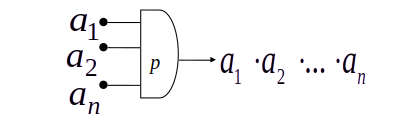
\includegraphics[scale=0.5]{графика/and.png}
\end{figure}

OR-элемент:

\begin{figure}[H]
    \centering
    \includegraphics[scale=0.5]{графика/or.png}
\end{figure}

\textbf{Теорема 1}. Суммирование двух $n$-разрядных двоичных чисел реализуется ПС сложности $9n-5$, которая обозначается $S_n$ и называется \textit{сумматором} порядка $n$.

\textbf{Теорема 2}. Умножение двух $n$-разрядных двоичных чисел реализуется ПС сложности $O(n^{log_2 3})$, которая обозначается $M_n$ и называется \textit{умножителем} порядка $n$.
\chapter{19 апреля. Логическое следование алгебры предикатов}
\section{Логическое следование формул алгебры предикатов}
$\vDash \Phi$ --- истинное утверждение при любой интерпретации.

$M = (M, \{P_M\}, \alpha)$, где $M \neq \varnothing$, $\alpha: X \to M$. --- интерпретация.

$\Phi_1, \dots, \Phi \vDash \Phi_\alpha$ --- из истинности $\Phi_1, \dots, \Phi$ следует истинность $\Phi_\alpha$ при любой интерпретации.

В алгебре высказываний у нас была единственная интерпретация $M = \{0,1\}$.

С помощью логического следования формул определяются общие способы доказательства взаимосвязи между истинностными значениями утверждений посредством исследования формальной структуры этих утверждений.

\dftion Формула $\Phi$ алгебры предикатов называется {\it логическим следствием } формулы $\Psi$, если $\vDash \Psi \then \Phi$, т. е. в любой интерпретации $M$ формула $\Phi$ истинна при любой оценке предметных переменных $\alpha$, при которой истинна формула $\Psi$.

\dftion Формула $\Phi$ называется {\it логическим следствием множества формул $\Gamma$}, если в любой интерпретации $M$ формула $\Phi$ истинна при любой оценке предметных переменных $\alpha$, при которой истинны все формулы из $\Gamma$.

Такое логическое следствие обозначается $\Gamma \vDash \Phi$ и называется {\it логическим следованием}. При этом формулы из $\Gamma$ называются {\it посылками} и формула $\Phi$ --- следствием логического высказывания.

\dftion Множество формул $\Gamma$ называется {\it проитиворечивым}, если из него логически следует любая ( в том числе и тождественно ложная) формула $\Phi$. Символически это записывается $\Gamma \vDash $.

\underline{Лемма 1 (Критерии логического следования).} Условие $\Phi_1, \dots, \Phi_m \vDash \Phi$ равносильно каждому из следующих условий:
\begin{itemize}
    \item $\Phi_1 \land \dots \land \Phi_m \vDash \Phi$
    \item $\vDash \Phi_1 \land \dots \land \Phi_m \then \Phi$
    \item $\Phi_1, \dots, \Phi_m, \neg \Phi \vDash $
\end{itemize}

В частности, $\Phi \vDash \Psi$ равносильно $\vDash \Phi \then \Psi$. Отсюда также следует, что $\Phi = \Psi$ Равносильно тому, что $\Phi \vDash \Psi$, $\Psi \vDash \Phi$.

\section{Проблема общезначимости формул алгебры предикатов}
Определение истинности формул вводится с помощью их интерпретаций в конкретных допустимых множествах $M$ с первоначально фиксированными предикатными символами этих формул. Так как множество таких интерпретаций бесконечно (они могут иметь как конечные, так и бесконечные области интерпретации), то в этом случае проверить тождественную истинность рассматриваемой формулы на всех таких интерпретациях практически невозможно.

Альтернативный подход к проверке общезначимости формулы $\Phi$ основывается на попытке построения интерпретации, опровергающей данную формулу.

Если из предположения существоввания такой интерпретации получается противоречие, то формула $\Phi$ общезначима. В противном случае на основе полученных условий для входящих в формулу $\Phi$ предикатов, алгебраических операций и констант строится интерпретация, опровергающая эту формулу $\Phi$, и в этом случае формула $\Phi$ не является общезначимой.

\section{Автоматическое доказательство теорем}
Мы будем проверять тождественную ложность. Суть в том, что мы будем идти через метод от противного.

Существуют алгоритмы поиска доказательства, которые для общезначимых формул подтверждают, что эти формулы общезначимы, и для необщезначимых формул в общем случае не заканчивают свою работу.

Автоматические системы построения доказательств называют {\it пруверами} и предъявляют им следующие требования:
\begin{enumerate}
    \item корректность
    \item полнота 
    \item эффективность
\end{enumerate}

Примером такого алгоритма является метод резолюций. Отсюда начинается теория алгоритмов.

Альтернатива методу резолюций --- алгоритм проверки.

%\sout{Ых, не видно нихера...}

\section{Метод резолюций в алгебре предикатов}
Первым шагом метода резолюций в алгебре предикатов является приведение рассматриваемой формулы к специальным нормальным формам, которые аналогичны ДНФ и КНФ для формул алгебры высказываний (далее АВ).

Формула исчисления предикатов $\Phi$ находится {\it в предваренной или пренексной нормальной форме} (далее ПНФ), если она имеет вид $(K_1 x_1)\dots(K_n x_n)\Psi$, где $K_1,\dots,K_n$ --- некоторые кванторы и $\Psi$ --- бескванторная формула, находящаяся в КНФ. При этом последовательность кванторов $(K_1 x_1)\dots(K_n x_n)$ называется {\it кванторной приставкой} и формула $\Psi$ называется {\it конъюнктивным ядром} формулы $\Phi$.

\underline{Теорема 1.} Любая формула исчисления предикатов $\Phi$ логически равносильна формуле $\Phi'$, находящейся в ПНФ.

Такая формула $\Phi'$ называется {\it пренексной нормальной формулой} (сокращённо ПНФ) формулы $\Phi$.

\subsection{Элиминация кванторов существования}

Пусть замкнутая формула исчисления предикатов $\Phi$ назодится в ПНФ:
\begin{equation*}
    \Phi = (K_1 x_1)\dots(K_n x_n)\Psi,
\end{equation*}
где $K_1,\dots,K_n$ --- некоторые кванторы и $\Psi = \Psi(x_1,\dots,x_n)$ --- конъюнктивное ядро формулы $\Phi$, т. е. бескванторная формула со свободными переменными $x_1,\dots,x_n$, находящимся в КНФ.

В кванторной приствке формулы $\Phi$ можно удалить любой квантор существования $(\exists x_s)$ для $1 \leq s \leq n$ по следующему правилу:
\begin{enumerate}
    \item Если левее квантора существования $(\exists x_s)$ в формуле $\Phi$ не стоит никакой квантор обзности, то выбираем новый предметный символ $c$, заменяем этим символом $c$ все вхождения переменной $x_s$ в конъюнктивное ядро формулы $\Phi$ и вычёркиванием $(\exists x_s)$ из кванторной приставки формулы $\Phi$;
    \item если же левее квантора существования стоят кванторы общности $(\forall x_{s_1})\dots(\forall x_{s_n})$ для значений $1 \leq s_1 \leq \dots \leq s_m \leq s$, то выбираем $m$-арный функциональный символ $f$, заменяем все вхождения переменной $x_s$ в конъюнктивное ядро формулы $\Phi$ выражением $f(x_{s_1},\dots,x_[s_n])$ и вычёркиванием $(\exists x_s)$ из кванторной приставки формулы $\Phi$
\end{enumerate}

В результате такой замены всех кванторов существования в формуле $\Phi$ получим замкнутую ПНФ $\Phi'$, кванторная приставка которой получается из кванторной приставки формулы $\Phi$ удалением всех кванторов существования и которая содержит все новые символы --- функциональные или предметные.

При этом формула $\Phi$ выполнима или противоречива одновременно с формулой $\Phi'$.

Рассмотренный приём удаления квантора был введён Скулемом и называется {\it скулемизацией формул}. Вводимые в процессе скулемизации новые функциональные и предметные символы называются {\it функторами Скулема} или {\it скулемовскими функциями}.

Получннную в результате скулемизации замкнутую формулу $\Phi'$ называют {\it скулевской стандартной формулой} (ССФ).

\underline{Теорема 2.} Любая замкнутая формула исчисления предикатов $\Phi$ эффективно преобразуется (с помощью определённого алгоритма) в логически эквивалентную ей скулемовскую стандартную форму $\Phi'$, которая называется {\it скулемовской стандартной формой} (сокращённо ССФ) формулы $\Phi$.

При этом формула $\Phi$ выполнима или противоречива одновременно с её ССФ.

\underline{Пример.} Результатом скулемизации формулы
\begin{equation*}
    (\forall x)(\exists z)(\forall y)(\exists w)((\neg P(x) \lor R(y)) \land P(z) \land \neg R(w))
\end{equation*}
является следующая ССФ
\begin{equation*}
    (\forall x)(\forall y)\Bigg(\Big(\neg P(x) \lor R(y)\Big) \land P(f(x)) \lor \neg R(g(x, y))\Bigg)
\end{equation*}

\section{Метод Эрбрана}
Это метод доказательства противоречивости множества дизъюнктов посредством невозможности построения интерпретации в специальном множестве $H$ ({\it универсум Эрбрана}), при котором все ... истинны.

Эрбранов универсум --- это множество, состоящее из постоянных символов и функциональных выражений для этих символов.

Если мы доказываем, что в таком универсуме нет интерпретаций, мы доказываем, что множество $S$ противоречиво. \newline

Доказательство тождественной истинности замкнутой формулы  равносильно доказательству противоречивости её отрицания $\neg \Phi$.

Далее рассматривается задача доказательства противоречивости замкнутой формулы $\Phi$.

{\bf Правило 1.} Противоречивость замкнутой формулы алгебры предикатов $\Phi$ равносильна противоречивости её скулемовской стандартной формы $\Phi'$, которая является универсально замкнутой формулой
\begin{equation*}
    \Phi' = (\forall_{i_1}x_{i_1})\dots(\forall_{i_k}x_{i_k})\Psi
\end{equation*}
с конъюнктивным ядром $\Psi = D_1\land\dots\land D_m$, где $D_1,\dots,D_m$ --- некоторые дизъюнкты литер алгебры предикатов.

С другой стороны, универсально замкнутая формула $\Phi'$ противоречива в том и только в том случае, когда она невыполнима.

Доказательство противоречивости (т. е. невыполнимости) замкнутой формулы $\Phi$ сводится к доказательству невыполнимости множества дизъюнктов $S = \{D_1,\dots,D_m\}.$

Эрбран доказал, что при доказательстве невыполнимости такого множества формул $S$ можно ограничиться рассмотрением интерпретаций в одной специальной области интерпретации, которая называется эрбрановским универсумом и состоит из функциональных выражений от констант из $S$.

{\bf Правило 2.} Доказательство противоречивости формул алгебры предикатов сводится к доказательству противоречивости конечных множеств дизъюнктов $S$.

Для этого строится резолютивный вывод 0 из множества дизъюнктов $S$.

Резолютивный вывод --- это последовательность дизъюнкций, в которой строится резольвента формул. Резольвента применялась к двум дизъюнктам. Один дизъюнкт имеет пропорциональную переменную $x$, а другой имеет отрицание $\neg x$. Эти переменные называются контранными (противоположными) литерами (в алгебре высказываний литерами являются переменные или их отрицания). Применение резольвенты есть сокращение контранных литер.

\section{Унификаторы формул}

\underline{Пример.}

В алгебре высказываний контрарные литеры $X, \neg X$.

В алгбере предикатов литеры $P(a, y), \neg P(x,f(b))$ не являются контрарными, но при замере переменных $\theta = \left(\begin{matrix}x & y \\ a & f(b)\end{matrix}\right)$ получаем контрарные литеры $P(a, f(b)), \lnot P(a, f(b))$.

\dftion Элементы области интерпретации могут описываться не только с помощью предметных переменных, но и с помощью так называемых \textbf{термов} --- специальных выражений языка, которые индуктивно определяются следующим образом:
\begin{itemize}
    \item все предметные переменные и предеметные символы формулы являются термами,
    \item если $f$ --- $n$-арный функциональный символ формулы и $t_1,\dots,t_n$ --- термы, то выражение $f(t_1,\dots,t_n)$ является термом.
\end{itemize}

Пусть $S$ --- множество формул алгебры предикатов.

Обозначим $X_S, C_S$ и $F_S$ соответственно множества всех предметных переменных, предметных символов и функциональных символов, встреечающихся в формулах множества $S$. Пусть $A_S$ --- объединение множеств $X_S$ и $C_S$ с добавленным новым постоянным символом $a$, если $C_S = \varnothing$.

На множестве $A_S$ определяется множество всех термов $T_S$ множества $S$ с функциональными символами из множества $F_S$. В частности, каждая переменная $x \in X_S$ является термом из множества $T_S$ и, значит, $X_S \subset T_S$.

Отображения $\theta$ множества переменных $X_S$ в множество термов $T_S$ называются {\it подстановками} и обозначаются
\begin{equation*}
    \theta = \left(\begin{matrix}
        x_1 & \dots & x_n \\ t_1 & \dots & t_n
    \end{matrix}\right),
\end{equation*}
где $t_i = \theta(x_i)$ для всех $x_i \in dom\, \theta$, удовлетворяющих $\theta(x_i) \neq x_i (i = \overline{1,n})$.

Заменять таким образом мы можем только переменные. Мы берём переменные и заменяем их на термы.
\chapter{26 апреля. Унификаторы формул}
Пусть $S$ --- множество формул алгебры предикатов.

Обозначим $X_S, C_S$ и $F_S$ соответственно множества всех предметных переменных, предметных символов и функциональных символов, встреечающихся в формулах множества $S$. Пусть $A_S$ --- объединение множеств $X_S$ и $C_S$ с добавленным новым постоянным символом $a$, если $C_S = \varnothing$.

На множестве $A_S$ определяется множество всех термов $T_S$ множества $S$ с функциональными символами из множества $F_S$. В частности, каждая переменная $x \in X_S$ является термом из множества $T_S$ и, значит, $X_S \subset T_S$.

Отображения $\theta$ множества переменных $X_S$ в множество термов $T_S$ называются {\it подстановками} и обозначаются
\begin{equation*}
    \theta = \left(\begin{matrix}
        x_1 & \dots & x_n \\ t_1 & \dots & t_n
    \end{matrix}\right),
\end{equation*}
где $t_i = \theta(x_i)$ для всех $x_i \in dom\, \theta$, удовлетворяющих $\theta(x_i) \neq x_i (i = \overline{1,n})$.

Действие подстановки $\theta$ естественно продолжается на термы из $T_S$, атомарные формулы, встречающихся в формулах множества $S$, и дизъюнкты из $S$.

Например, для терма $t=t(x_1,\dots,x_n)$ значение $\theta(t) = t(\theta(x_1), \dots, \theta(x_n))$.

Аналогично, для формулы $D$ значение $\theta(D)$ есть формула, полученная заменой всех вхождений в $D$ термов $t$ на термы $\theta(t)$.

Пусть $W=\{\Phi_1,\dots,\Phi_k\}$ --- множество атомарных формул, встречающихся в формулах из множества $S$. Подстановка $\theta$ называется \textit{унификатором множества формул} $W$, если $\theta(\Phi_1) = \dots = \theta(\Phi_k$).

Говорят, что множество атомарных формул $W$ \textit{унифицируемо}, если для него существует унификатор.

\underline{Пример}. Множество формул $\{P(b, y), P(x, f(c))\}$ с бинарным предикатным символом $P$, унарным предикатным символом $f$ и предметными символами $b, c$, так как подстановка $\theta = \left(
    \begin{matrix}
        x & y \\
        b & f(c)
    \end{matrix}
\right)$ является его унификатором.

\section{Резольвенты и резолютивный вывод в исчислении предикатов}
Пусть $S$ --- множество дизъюнктов, $D_1, D_2$ --- дизъюнкты из $S$, которые \underline{не имеюот общих переменных}, и $L_1, L_2$ --- литеры в $D_1$ и $D_2$ соответственно.

Если множество формул $W=\{L_1, \lnot L_2\}$ имеет унификатор $\theta$, то дизъюнкт, получаемый из дизъюнкта $\theta(D_1) \lor \theta(D_2)$ вычёркиванием литер $\theta(L_1)$ и $\theta(L_2)$, называется \textit{бинарной резольвентой} дизъюнктов $D_1$ и $D_2$ и обозначается символом $res(D_1, D_2)$. При этом литеры $L_1$ и $L_2$ называются \textit{отрезаемыми литерами}.

Если $\theta(D_1) = \theta(L_1)$ и $\theta(D_2) = \theta(L_2)$, то бинарную резольвенту дизъюнктов $D_1$ и $D_2$ полагаем равной 0.

Если дизъюнкты $D_1$, $D_2$ имеют общие переменные, то, заменив в формуле $D_2$ эти общие переменные на переменные, не встречающиеся в $D_1$ и $D_2$, получим дизъюнкт $D_2'$, который не имеет общих переменных с дизъюнктом $D_1$.

\textit{Бинарной резольвентой} дизъюнктов $D_1$ и $D_2$ называется бинарная резольвента дизъюнтов $D_1$ и $D_2'$.

\underline{Пример}. Найдём бинарную резольвенту дизъюнктов $d-1 = P_1(x) \lor P_2(x)$ и $D_2 = \lnot P_1(c) \lor P_3(x)$.

Так как $D_1, D_2$ имеют общую переменную $x$, то заменим в формуле $D_2$ $x$ на новую переменную $y$: $D_2 = \lnot P_1(c) \lor P_3(y)$.

Выбираем в $D_1$ и $D_2$ литеры $L_1 = P_1(x)$ и $L_2 = \lnot P_1(c)$ соответственно. Так как $\lnot L_2 = L_2 = P_1(c)$ и формулы $L_1, L_2$ имеют унификатор $\sigma = \left(
    \begin{matrix}
        x \\
        c
    \end{matrix}
\right)$, то бинарная резольвента формул $D_1$ и $D_2$ получается из $\sigma(D_1) \lor \sigma(D_2')=P_1(c)\lor P_2(c)\lor\lnot P_1(c) \lor P_3(y)$ вычёркиванием литер $P_1(c)$ и $\lnot P_1(c)$.

\dftion \textbf{Резолютивный вывод} формулы $\Phi$ из множества дизъюнктов $S$ есть такая конечная последовательность дизъюнктов $\Phi_1,\dots,\Phi_k$, что
\begin{enumerate}
    \item $\Phi_k = \Phi$,
    \item каждый дизъюнкт $\Phi_i$ или принадлежит множеству $S$, или является резольвентой некоторых дизъюнктов, предшествующих $\Phi_i$
\end{enumerate}

\textbf{Лемма}. Резолютивный вывод из множества дизъюнктов $S$ сохраняет выполнимость формул.

\textbf{Правило 3 (основная теорема метода резолюций)}.
Множество дизъюнктов $S$ противоречиво тогда и только тогда, когда существует резолютивный вывод нуля из $S$.

\underline{Пример}. Докажем противоречивость множества дизъюнктов $W = \{\Phi_1, \dots, \Phi_6\}$, где
\begin{itemize}
    \item $\Phi_1 = P_1(a, f(b), f(c))$
    \item $\Phi_2 = P_2(a)$
    \item $\Phi_3 = P_1(x, x, f(x))$
    \item $\Phi_4 = \lnot P_1(x, y, z) \lor P_3(x, z)$
    \item $\Phi_5 = \lnot P_2(x) \lor \lnot P_1(y, z, u) \lor \lnot P_3(x, u) \lor P_3(x, y) \lor P_3(x, z)$
    \item $\Phi_6 = \lnot P_3(a, c)$
\end{itemize}
Выполним резолютивный вывод:
\begin{enumerate}
    \item $\Phi_7 = res(\Phi_2, \Phi_5) = res(\Phi_2, \left(
        \begin{matrix}
            x & y \\
            a & z
        \end{matrix}
    \right)(\Phi_5)) = \lnot P_1(z, z, u) \lor \lnot P_3(a, u) \lor P_3(a, z)$
    \item $\Phi_8 = res(\Phi_3, \Phi_7) = res(\Phi_3, \left(
        \begin{matrix}
            z & u \\
            x & f(x)
        \end{matrix}
    \right)(\Phi_7)) = \lnot P_3(a, f(x)) \lor P_3(a, x)$
    \item $\Phi_9 = res(\Phi_6, \Phi_8) = res(\Phi_6, \left(
        \begin{matrix}
            x \\
            c
        \end{matrix}
    \right)(\Phi_8)) = \lnot P_3(a, f(c))$
    \item $\Phi_{10} = res(\Phi_4, \Phi_9) = res(\left(
        \begin{matrix}
            x & z \\
            a & f(c)
        \end{matrix}
    \right)(\Phi_4), \Phi_9) = \lnot P_1(a, y, f(c))$
    \item $\Phi_{11} = res(\Phi_1, \Phi_{10}) = res(\Phi_1, \left(
        \begin{matrix}
            y \\
            f(b)
        \end{matrix}
    \right)(\Phi_{10})) = 0$
\end{enumerate}

\section{Применения метода резолюций исчислении предикатов}
Следующие задачи равносильны:
\begin{itemize}
    \item проверка тождественной истинности формул
    \item проверка логического следования формул
    \item проверка тождественной ложности формул
    \item проверка противоречивости множества формул
    \item проверка противоречивости множества дизъюнтов
\end{itemize}

\section{Алгоритм метода резолюций в исчислении предикатов}
\begin{enumerate}
    \item Доказательство тождественной истинности формулы $\Phi$ сводится к доказательству протиоречивости её отрицания $\Psi = \lnot \Phi$.
    \item Доказательство противоречивости замкнутой формулы алгебры предикатов $\Psi$ сводится к доказательству противоречивости её скулемовской стандартной формы (ССФ) $\Psi'$, которая является универсально замкнутой формулой $$\Psi' = (\forall x_i) \dots \Psi''$$ с конъюнктивным ядром $$\Psi'' = D_1 \land \dots \land D_M,$$ где $D_1,\dots,D_m$ --- некоторые дизъюнкты литер алгебры предикатов.
    \item Доказательство противоречивости ССФ $\Psi'$ с конъюнктивным ядром $$\Psi'' = D_1 \land \dots \land D_M$$ сводится к доказательству противоречивости конечного множества дизъюнтов $$S = \{D_1,\dots,D_M\}$$ путём построения резолютивного вывода $0$ из множества дизъюнктов $S$.
    \item Если построен резолютивный вывод 0 из множества дизъюнктов $S$, то по основной теореме метода резолюций множество дизъюнктов $S$ противоречиво и исходная формула $\Phi$ тождественно истинна
\end{enumerate}

\underline{Пример}. Методом резолюций доказать общезначимость формулы
$$\Phi = \Big((\exists x)P(x) \then (\forall x)R(x)\Big)\then(\forall x)(P(x) \then R(x))$$
\begin{enumerate}
    \item Условие $\vDash \Phi$ равносильно $\lnot \Phi \vDash$
    \item Для формулы $\Psi = \lnot \Phi$ найдём ПНФ и ССФ. ПНФ формулы $\Psi$ будет $$(\forall x)(\forall y)(\exists z)\Bigl(\bigl(\lnot P(x) \lor R(y)\bigr)\land P(z) \land \lnot R(z)\Bigr),$$ а ССФ --- $$(\forall x)(\forall y)\Bigl(\bigl(\lnot P(x) \lor R(y)\bigr)\land P(f(x,y)) \land \lnot R(f(x,y))\Bigr)$$
    \item Для доказательства невыполнимости этой формулы доказываем противоречивость множества дизъюнктов её конъюнктивного ядра $$S=\{\lnot P(x) \lor R(y), P(f(x, y)), \lnot R(f(x,y))\}$$
\end{enumerate}
Резолютивный вывод формулы 0 из множества дизъюнктов $S$:
\begin{itemize}
    \item $\Phi_1 = \lnot P(x) \lor R(y)$
    \item $\Phi_2 = P(f(x, y))$
    \item $\Phi_3 = res(\Phi_1, \Phi_2) = res(\lnot P(x) \lor R(y), P(f(x, y))) = res(\lnot P(x) \lor R(y), P(f(x_1, y_1))) = res(\lnot P(f(x_1, y_1)) \lor R(y), P(f(x_1, y_1))) = R(y)$, где $\theta = \left(
        \begin{matrix}
            x \\
            f(x_1, y_1)
        \end{matrix}
    \right)$
    \item $\Phi_4 = \lnot R(f(x_y))$
    \item $\Phi_5 = res(\Phi_3, \Phi_4) = res(R(y), \lnot R(f(x, y))) = res(R(y), \lnot R(f(x_1, y_1))) = res(\theta(R(y)), \lnot R(f(x_1, y_1))) = res(R(f(x_1,y_1)), \lnot R(f(x_1, y_1))) = 0$, где $\theta = \left(
        \begin{matrix}
            y \\
            f(x_1, y_1)
        \end{matrix}
    \right)$
\end{itemize}
\chapter{3 мая. Аксиоматический метод}
Было определено множество формул алгебры высказываний $F_{AB}$.

Затем было выделено подмножество формул $T_{AB} \subset F_{AB}$, состоящее из специальных формул --- тавтологий.

При этом в основе определения тавтологии лежит понятие интерпретации формул, то есть придание некоторого конкретного содержательного смысла входящих в них переменных. Такой подход к логическим формулам носит теоретико-множественный характер и называется \textit{семантическим}.

Альтернативой семантического подхода является \textit{синтаксический подход}, при котором логические формулы выводятся из первоначально выделенного множества формул --- аксиом --- по определённым правилам преобразования формул логического языка без привлечения вспомогательных теоретико-множественных понятий.

Построение математических теорий в виде аксиоматических теорий соответствующих формальных исчислений составляет суть \textit{аксиоматического метода в математике}.

Простейшей аксиоматической теорией является \textit{аксиоматическая логика высказываний}, которая строится на основе соответствующего формального исчисления, называемого \textit{исчислением высказываний} (сокращённо ИВ).

\section{Исчисление высказываний}
Множество аксиом Ax(ИВ) исчисления высказываний описывается следующими тремая \textit{схемами аксиом}:
\begin{enumerate}
    \item $(A_1)$ $(\Phi \then (\Psi \then \Phi))$,
    \item $(A_2)$ $((\Phi_1 \then (\Phi_2 \then \Phi_3)) \then ((\Phi_1 \then \Phi_2) \then (\Phi_1 \then \Phi_3)))$,
    \item $(A_3)$ $((\lnot \Phi \then \lnot \Psi)\then ((\lnot \Phi \then \Psi)\then \Phi))$,
\end{enumerate}
где $\Phi, \Psi, \Phi_i$ ($i = \overline{1,3}$) --- произвольные формулы исчисления высказываний.

Исчисление высказываний имеет \textbf{правило вывода}, которе называется \textbf{правилом заключения} или правилом \textit{modus ponens} (сокращённо MP) и которое для произвольных формул исчисления высказываний $\Phi, \Psi$ определяется по формуле MP $(\Phi \then \Psi, \Phi) = \Psi$.

Символически это правило вывода записывается следующей схемой:
\begin{equation*}
    MP: \begin{matrix}
        \Phi \then \Psi, \Phi \\
        \Psi
    \end{matrix}.
\end{equation*}

В основе алгоритма вывода \textbf{теорем} исчисления высказываний лежит следующее понятие.

\dftion Формула $\Phi$ называется \textit{теоремой исчисления высказываний}, если найдётся такая конечная последовательность формул $\Phi_1, \dots, \Phi_n$, в которой:
\begin{enumerate}
    \item $\Phi_n = \Phi$
    \item каждая формула $\Phi_i$ либо являтся аксиомой, либо получается из некоторых двух предыдущих формул $\Phi_i, \Phi_k$ ($1 \leq j, k < i$) по правилу вывода MP.
\end{enumerate}

Последовательность формул $\Phi_1, \dots, \Phi_n$ называется \textbf{выводом} или \textbf{доказательством} формулы $\Phi$.

\dftion Вывод формулы $\Phi$ сокращённо обозначают символом $\vdash \Phi$ и говорят, что $\Phi$ есть теорема. Множество всех таких теорем обозночается символом Th(ИВ) и называется \textbf{теорией исчисления высказываний}.

Главной целью построения исчисления высказываний является определение такой теории Th(ИВ), которая совпадает с множеством тавтологий $T_{AB}$.

\textbf{Лемма}.
Справедливы следующие утверждения:
\begin{enumerate}
    \item всякая аксиома ИВ является тавтологией;
    \item результат применения правила вывода MP к люым тавтологиям $\Phi \then \Psi, \Phi$ даёт тавтологию $\Psi$;
    \item всякая теорема ИВ является тавтологией, то есть выполняется $Th(\text{ИВ}) \supset T_{\text{АВ}}$.
\end{enumerate}

\textbf{Теорема полноты ИВ}.
Всякая тавтология является теоремой ИВ, т. е. выполняется $T_\text{АВ} \subset Th(\text{ИВ})$ и, следовательно, $T_{AB}=Th(\text{ИВ})$.

Следствия теоремы полноты ИВ.

\textbf{Теорема о непротиворечивости ИВ}.

В исчислении высказываний невозможно доказать никакую формулу $\Phi$ вместе с её отрицанием $\lnot \Phi$.



\textbf{Теорема о разрешимости ИВ}.
Существует универсальная эффективная процедура (алгоритм), которая для любой формулы определяет, является ли эта формула теоремой ИВ.

\section{Исчисление предикатов}
Множество аксиом Ax(ИП) исчисления предикатов описываетя пятью \textit{схемами аксиом} --- тремя определёнными в предыдущем разделе схемами схемами $(A_1)-(A_3)$, в которых $\Phi, \Psi, \Phi_i (i = \overline{1,3})$ являются произвольными формулами исчисления предикатов, и двумя новыми схемами:
\begin{enumerate}
    \setcounter{enumi}{3}
    \item $(A_4)$ $(\forall x)\Phi(x) \then \Phi(y)$ для произвольной формулы $\Phi(x)$, в которую $y$ не входит связно;
    \item $(A_5)$ $(\forall x)(\Phi \then \Psi(x)) \then (\Phi \then (\forall x)\Psi(x))$ для таких формул $\Phi, \Psi$, что $x$ в формулу $\Phi$ не входит свободно.
\end{enumerate}

Исчисление предикатов имеет два \textbf{правила вывода} --- правило modus ponens (сокращнно MP) и правило обобщения (сокращённо Gen), которые для произвольных формул исчисления предикатов $\Phi, \Psi$ символически записываются следующими схемами:
\begin{figure}[H]
    \centering
    \begin{tabular*}{0.5\textwidth}{@{\extracolsep{\fill}}ccc@{}}
        $MP: \begin{matrix}
            \Phi \then \Psi, \Phi \\
            \Psi
        \end{matrix}$ &
        и &
        $Gen: \begin{matrix}
            \Phi \\
            (\forall x)\Phi
        \end{matrix}$.
    \end{tabular*}
\end{figure}

\dftion Формула $\Phi$ называется \textbf{теоремой исчисления предикатов}, если найдётся такая последовательность $\xses[\Phi]$, в которой $\Phi_n = \Phi$ и каждая формула $\Phi_i$ либо является аксиомой, либо получается из некоторых предыдущих формул этой последовательности по одному из правил вывода MP или Gen. При этом $\Phi_1, \dots, \Phi_n$ называется \textbf{выводом} или \textbf{доказательством} формулы $\Phi$.

Вывод формулы $\Phi$ обозначают $\vdash \Phi$ и говорят, что $\Phi$ есть теорема. Множество всех таких теорем обозначается символом Th(ИП) и называется \textit{теорией исчисления предикатов}.

Цель построения исчисления предикатов --- определение такой теории Th(ИП), которая совпадает со множеством тавтологий $T_{\text{АП}}$.

\textbf{Лемма 1}.
Справедливы следующие утверждения:
\begin{enumerate}
    \item всякая аксиома ИП является тавтологией;
    \item результат применения правил вывода MP и Gen к тавтологиям является тавтологией;
    \item любая теорема ИП является тавтологией ИП, т. е. имеет место включение $Th(\text{ИП}) \supset T_{\text{АП}}$.
\end{enumerate}

Доказательство $T_{\text{АП}} \subset Th(\text{ИП})$ был получено астрийским математиком К. Геделем в 1930 году.

\textbf{Теорема полноты ИП}.

Формула исчисления предикатов в том и только в том случае является тавтологией, если она есть теорема ИП, т. е. выполняется равенство $T_{\text{АП}}=Th(\text{ИП})$.

Таким образом, ИП является адекватным инструментом получения логических законов.

\textbf{Теорема о непротиворечивости ИП}
В исчислении предикатов невозможно доказать никакую формулу $\Phi$ вместе с её отрицанием $\lnot \Phi$.

С другой стороны, английский математик А. Черч в 1936 году доказал следующий принципиально важный результат.

\textbf{Теорема о неразрешимости ИП}.

Не существует универсальной эффективной процедуры (алгоритма), которая для любой формулы определяет, является ли эта формула теоремой ИП.

\section{Элементы теории алгоритмов}
Важные математические проблемы имеют вид:

для некоторого данного множества $X$ найти эффективную процедуру (т. е. алгоритм), с помощью которой можно для каждого элемента $x$ этого множества $X$ определить за конечное число шагов, будет этот элемент обладать некоторым данным свойством $P$ или нет (т. е. $x \in P^+$ или $x \not\in P^+$).

\textit{Решение} такой проблемы --- построение и обоснование искомого алгоритма.

\dftion \textbf{Массовые задачи} --- задачи распознавания и оптимизации.

Примеры массовых задач:
\begin{itemize}
    \item ВЫП (SAT) --- задача выполнимости формулы логики высказываний
    \item ТЕОРЕМА (THM) --- задача доказуемости формулы логики предикатов
\end{itemize}
\chapter{10 мая. Элементы теории алгоритмов}
\section{Унификация разнородной задачи}
\underline{Определение распознавательной задачи}

Имеется множество объектов $X$ и определённое подмножество $P \subset X$, требуется найти эффективную процедуру (т. е. алгоритм), с помощью которой для любого $x \in X$ можно определить $x \in P$ или $x \not\in P$.

\dftion При этом распознавательная задача называется \textbf{алгоритмически разрешимой} или \textit{алгоритмически неразрешимоой} в зависимости от того, имеется или нет алгоритм решения этой задачи.

Чем более массовый алгоритм, тем лучше.

Конструктивные объекты любого множества $X$ можно \textit{кодировать} словами конечного множества $\Sigma$ (например, состоящего из двоичных символов 0 и 1) с помощью взаимно-однозначного отображения $f: X \to \Sigma*$, где $\Sigma*$ --- множество всех слов над алфавитом $\Sigma$.

Подмножества множества всех слов $L \subset \Sigma*$ --- языки над алфавитом $\Sigma$.

\underline{Пример}. Кодировка проблемы выполнимости (ВЫП).

\textit{Формулы алгебры высказыаний} строятся из следующих элементов.

\begin{enumerate}
    \item Пропозициональные переменные, принимающие значения 1 (истина) или 0 (ложь)
    \item Бинарные операторы $\land$, $\lor$, обозначающие логические связки И, ИЛИ двух формул
    \item Унарный оператор $\lnot$, который обозначает логическое отрицание
    \item Скобки для группирования операторов и операндов, если необходимо изменить порядок старшинства (приоритетов) операторов, принятый по умолчанию (вначале применяется $\lnot$? затем $\land$ и, наконец, $\lor$).
\end{enumerate}

$\Sigma = \{0, 1, \land, \lor, \lnot, (, ), X\}$

$\forall x \in X \; \Phi \to f(\Phi) \in \Sigma^*$

$X_i = \{f(\phi): \phi ~ \text{--- выполнимая формула}\}$

$W \in f(\Gamma_{\text{АВ}})$

Для кодировки экземпляров ВЫП используется следующий код.
\begin{enumerate}
    \item Символы $\land$, $\lor$, $\lnot$ и скобки $($,$)$ представляют самих себя
    \item Переменная $X_i$ представляется символом $X$ с дописанной к нему последовательностью нулей и единиц --- двоичной записью числа $i$
\end{enumerate}

Таким образом, алфавит $\Sigma$ проблемы-языка ВЫП содержит всего восемь символов. Все экземпляры ВЫП являются цепочками символов --- словами в этом фиксированном конечном алфавите. Множество кодов всех формул алгбры высказываний образует подмножество $W \subset \Sigma*$ и множество всех выполнимых формул алгебры высказываний образует подмножество $L \subset W$. Требуется найти эффективную процедуру (т. е. алгоритм), с помощью которой для любого слова $w \in W$ можно определить $w \in L$ или $w \not\in L$.

\section{Интуитивное понятие алгоритма и его математические модели}
\dftion Под \textbf{алгоритмом} интуитивно понимается совокупность инструкций, которые дают решение некоторой массовой задачи.

Общие свойства алгоритма:
\begin{enumerate}
    \item дискретность алгоритма
    \item детерменированность алгоритма
    \item элементарность шагов алгоритма
    \item массовость алгоритма
\end{enumerate}

Множество слов для алфавита $\Sigma = \{0, 1\}$ имеет вид:
$$ \Sigma* = \{\land, 0, 1, 00, 01, 10, 11, \dots \}, $$
где $\land$ --- пустое слово (его наличие подразумевается, когда множество слов обозначается символом *).

Так как конструктивные объекты можно кодировать словами конечного алфавита $\Sigma$ (например, состоящего из двоичных символов 0 и 1), то алгоритм моделируется устройством, перерабатывающим слова алфавита $\Sigma$.

\textbf{Тезис Черча}.

Класс задач, решаемых в любой формальной модели алгоритма, совпадает с классом задач, которые могут быть решены интуитивно эффективными вычислениями, то есть алгоритмическими методами.

Алгоритмически неразрешимые задачи привели к необходимости строго математического определения алгоритма.

\dftion Основные варианты математического определения алгорима --- \textbf{модели алгоритма}:
\begin{enumerate}
    \item Понятие \textit{рекурсивной функции}, введённое Клини в 1936 году
    \item Понятие \textit{машины Тьюринга}, введённое Постом и Тьюрингом в 1936 году
    \item Понятие \textit{нормального алгорифма}, введённое Марковым в 1954 году
    \item Понятие \textit{формальной грамматики}, введённое Хомским в 1957 году
\end{enumerate}

\section{Машины Тьюринга}
\subsection{Логическое описание}
Реализация модели вычислений с помощью понятия машины Тьюринга.

При построении математической модели алгоритма Пост и Тьюринг исходили из того, что все действия, которые может производить любой алгоритм, можно разложить на некоторые канонические элементарные шаги, выполняемые подходяще устроенными вычислительными машинами.

Такие машины схематически определяются следующим образом:

\begin{figure}[H]
    \centering
    
\includegraphics[scale=0.25]{графика/тьюринг.png}
\end{figure}

\begin{enumerate}
    \item Символы внешнего алфавита $\Sigma = \{0,1,\dots\}$ записываются в ячейки конечной ленты, которя называется \textbf{внешней памятью машины}, при необходимости в ячейки записывается символ *, который называется \textit{пустым}
    \item Символы внутреннего алфавита $Q=\{q_S,q_F,\dots\}$ обозначают состояния \textbf{управляющего устройства машины} (УУ) с \textbf{просматривающей головкой}, которая может перемещаться вдоль ленты и в каждый момент времени $t$ просматривать одну ячейку
    \item \textbf{Программа машины} $$\Pi = \{T(q,a:q\in Q \backslash \{q_F\} \land a \in \Sigma)\}$$ состоит из \textbf{команд} $T(q, a) = qa \to q'a'X$, которые в зависимости от состояния машины $q$ и символа $a$ в просматриваемой ячейке УУ заменяют в этой ячейке букву $a$ на букву $a'$, состояние $q$ на состояние $q'$ и в зависимости от значения $X \in \{R, L, S\}$ сдвигают просматривающую головку либо в соседнюю правую ячейку при $X = R$, либо в соседнюю левую ячейку $X = L$, либо оставляет головку на месте при $X = S$. При необходимости на ленте достраиваются справа или слева ячейки с пустым символом $*$
    \item Машина начинает работать в \textbf{начальном состоянии} $q_S$ и заканчивает работать в \textbf{заключительном} состоянии $q_F$
\end{enumerate}

Вход машины: слово $w \in \Sigma*$ на ленте машины $T$ в начальном состоянии $q_S$.

Выход машины: слово $s' \in \Sigma*$ на ленте машины $T$ в заключительном состоянии $q_F$.

Строго математически такие машины определяются следующим образом.

\subsection{Математическое описание машины Тьюринга}
\dftion \textbf{Машина Тьюринга} $T$ представляет собой алгебраическую систему $T = (\Sigma, Q, \delta, q_S, q_F)$, работающую в дискретные моменты времени $t=0,1,2\dots$ и состоящую из следующих частей:

\begin{itemize}
    \item Конечное множество $\Sigma=\{0,1\dots\}$ называется \textit{внешним алфавитом}
    \item Конечное множество $Q = \{q_S, q_F, \dots\}$ называется \textit{внутренним алфавитом}, элементы $Q$ называются \textit{состояниями машины}
    \item Отображение $\delta: Q \times \Sigma \to Q \times \Sigma \times \{R, L, S\}$, которое определяет список команд $T(q, a) = qa \to q'a'X$ --- символическое оюозначение образов $\delta(q, a) = (q', a', X)$ отображения $\delta$ для $q \in Q \backslash \{q_F\}, a \in \Sigma$ и $X \in \{R, L, S\}$, множество всех команд $\Pi = \{T(q, a): q \in Q \backslash \{q_F\} \land a \in Sigma\}$ называется \textit{программой машины}
    \item Состояние $q_S$ называется \textit{начальным} и означает начало работы машины
    \item Состояние $q_F$ называется \textit{заключительным} и означает завершение работы машины
\end{itemize}

Работа машины Тьюринга $T$ происходит под действием её команд и заключается в измений её \textit{конфигураций}, описывающих состояния ленты и управляющего устройства, а также положение головки относительно ячеек ленты: если лента находится в состоянии, которое описывается словом $\alpha a \beta$ над алфавитом $\Sigma$, и головка в состоянии $q$ просматривает на ленте ячейку с состоянием $a$, то соответствующая конфигурация $K$ машины $T$ описывается выражением $M=\alpha q a \beta$, которое называется \textbf{машинным словом}.

При этом $K$ называется \textbf{начальной конфигурацией}, если описывающее её машинное слово содержит символ начального состояния $q_S$, и \textbf{заключительной конфигурацией}, если описывающее её машинное слово содержит символ заключительного состояния $q_F$.

Программа указывает, что машина делает в каждый момент времени в зависимости от её настоящей конфигурации $K$:
\begin{itemize}
    \item Если $K$ --- заключительная конфигурация, то машина заканчивает работу
    \item Если K не является заключительной конфигурацией и описывается машинным словом $M=\alpha q a \beta$, то в программе $\Pi$ машина находит команду $T(q, a)$ с левой частью $qa$ и в зависимости от вида правой части такой команды $T(q,a)$ машина заменяет в просматриваемой ячейке букву $a$ на букву $a'$, состояние $q$ на состояние $q'$ и в зависимости от значения $X \in \{R, L, S\}$ сдвигают просматривающую головку либо в соседнюю правую ячейку при $X = R$, либо в соседнюю левую ячейку при $X = L$, либо оставляет головку на месте при $X = S$
\end{itemize}

Изменение конфигруаций $K_0, K_1, K_2, \dots$ машины $T$ под действием команд происходит в дискретные моменты времени $t = 0, 1, 2, \dots$ и описывается преобразованием соответствующих машинных слов $M_0, M_1, M_2, \dots$ по следующему правилу. За один шаг работы машины $T$ её машинное слово $M = \alpha q a \beta$ под действием команды $T(q ,a)$ преобразуется в новое машинное слово $M'$ по формулам:
\begin{itemize}
    \item если $T(q,a) = qa \to q'a'S$, то $M' = \alpha q' a' \beta$
    \item если $T(q, a) = qa \to q'a'R$ и $M = \alpha q a b \beta'$, то $M' = \alpha a'q'b\beta'$
    \item если $T(q,a) = qa \to q'a'R$ и $M=\alpha q a$, то $M' = \alpha a' q' *$
    \item если $T(q,a) = qa \to q'a'R$ и $M = \alpha q a$, то $M' = \alpha a' q' *$
    \item если $T(q, a) = qa \to q' a'L$ и $M=\alpha'bqa\beta$, то $M'=\alpha'q'ba'\beta$,
    \item если $T(q,a) =  qa \to q'a'L$ и $M = qa\beta$, то $M' = q'*a'\beta$
\end{itemize}

Символически такое одношаговое преобразование машинных слов обозначается $M \to^T M'$.

Если существует такая последовательность преобразований машинных слов $M_i \to^T M_{i+1}$ (где $i = 0,1,\dots,k-1$), для которой $M_0 = M$ и $M_k = M'$, то пишут $M \then^T M'$ и говорят, что машинное слово $M'$ получается из машинного слова $M$ с помощью машины $T$.

\dftion \textbf{Вход} (начало работы) машины: слово $w \in \Sigma*$ на ленте машины $T$ в начальном состоянии $q_S$.

\dftion \textbf{Выход} (завершение работы) машины: слово $w' \in \Sigma*$ на ленте машины $T$ в заключительном состоянии $q_F$.

В этом случае говорят, что машина $T$ \textbf{принимает} слово $w$ и выдаёт значение $w'=T(w)$. В результате машина $T$ определяет язык $L(T)\subset\Sigma*$, который состоит из всех принимаемых машиной $T$ слов.

\dftion Язык $L \subset \Sigma*$ \textbf{принимается} машиной Тьюринга, если $L=L(T)$ для некоторой машины Тьюринга $T$.

Таким образом, любая машина Тьюринга $T$ определяет частичную функцию $f$ из $\Sigma*$ в $\Sigma*$, область определения которой $D_f$ состоит из всех слов алфавита $\Sigma$, которые принимает машина $T$, и значения которой для слов $w \in D_f$ определяются по формуле: $f(w) = T(w)$.

\dftion Частичная фунция $f$ из $\Sigma*$ в $\Sigma*$ называется \textbf{вычислимой по Тьюрингу}, если она определяется некоторой машиной Тьюринга.

\underline{Пример}. Пусть машина Тьюринга $T$ имеет внешний алфавит $\Sigma=\{0,1\}$, внутренний алфавит $Q=\{q_S,q_F, q\}$ и программу $\Pi$, которая состоит из команд $q_S1\to q1R, q1\to q1R, q* \to q_F 1S$. Тогда слово $\alpha=11$ машиной $T$ перерабатывается в слово $\beta=111$, так как
$$ \underline{q_s1}1 \underset{(1)}\to^T 1\underline{q1} \underset{(2)}\to^T 11\underline{q*} \underset{(3)}\to^T 11\underline{q_F}1 ~ \text{и} ~ T(11) = 111. $$

Легко видеть, что любое слово $\alpha = 1^n$ над алфавитом $\Sigma=\{0, 1\}$ машиной $T$ перерабатывается в слово $\beta = \alpha 1 = 1^{n+1}$. Это означает, что машина $T$ к любому слову над алфавитом $A = \{1\}$ приписывает справа символ 1.

\dftion Частичная словарная функция $f:(\Sigma*)^n \to \Sigma*$ над алфавитом $\Sigma$ называется \textbf{вычислимой по Тьюрингу}, если существует машина Тьюринга $T$ с внешним алфавитом $\Sigma$, для которой при любых $w_1, \dots, w_n \in \Sigma*$ условие $(w_1, \dots, w_n) \in D_f$ равносильно тому, что машина $T$ применима к слову $\alpha = w_1 * \dots * w_n$ и результат $T(\alpha)$ переработки данной машиной $T$ такого слова равен значению функции $f(w_1,\dots,w_n)$.

\textbf{Основная теорема}.
Для любой частичной словарной функции $f: (\Sigma*)^n \to \Sigma*$ следующие условия эквивалентны:

\begin{enumerate}
    \item Функция $f$ вычислима по Тьюрингу
    \item Функция $f$ частично рекурсивна
    \item Функция $f$ нормально вычислима
\end{enumerate}

Такие вычислительные процедуры называются \textbf{алгоритмами}.

\section{Вычислимость: разрешимые и полуразрешимые языки}
\underline{Определение 1}. Язык $L$ называется \textit{разрешимым} (или \textit{рекурсивным}), если существует такая машина Тьюринга $T$, что для любого слова $w \in W$ выполняются условия:
\begin{itemize}
    \item если $w \in L$, то при входе $w$ машина $T$ попадает в заключительное состояние, останавливается и выдаёт значение $T(w) = 1$
    \item если $w \not \in L$, то при входе $w$ машина $T$ попадает в заключительное состояние, останавливаетс и выдаёт значение $T(w) = 0$
\end{itemize}

Такие машины соответствуют понятию <<алгоритма>> и применяются при решении \textit{распознавательных задач} типа <<да/нет>>.

Множество всех разрешимых языков будем обозначать $R$ (от Recursive).

\textbf{Свойства}: дополнения, конечные пересечения и конечные объединения разрешимыъх языков являются разрешимыми языками.

\textbf{Примеры разрешимых языков}.
\begin{itemize}
    \item Пустой языкМножество всех строк
    \item Конечные множества
    \item Множество чётных чисел
    \item Множество простых чисел
    \item Множество рациональных чисел, не превышающих $e$
    \item Множество всех чисел $n$, при которых в $\pi$ не меньше $n$ девяток подряд
\end{itemize}

\underline{Определение 2}. Язык $L$ называется \textit{полуразрешимым} или \textit{перечислимым}, если существует такая машина Тьюринга, что
\begin{equation}
    L = L(T) = \{w \in \Sigma* : T(w) = 1\},
\end{equation}
то есть при выходе $w \in L$ машина $T$ попадает в заключительное состояние, останавливается и выдаёт значение $T(w) = 1$, а при выходе $w \not \in L$\dots\dots\dots

\underline{Лемма}. Существуют неразрешимые языки, поскольку алгоритмов счётное число, а языков несчётное.

Аналогично можно доказать, что существуют языки, не являющиеся полуразрешимыми.

\underline{Основная теорема}. Существуют полуразрешимые неразрешимые языки, т. е. полуразрешимые языки, которые не могут быть разрешимы никакм алгоритмом, т. е. выполняется свойство $R \not \subset RE$.
\chapter{17 мая. Вычислимость}
\section{Вычислимость: разрешимые и полуразрешимые языки}
Распознавательная задача формулируется следующим универсальным образом: имеется множество слов $W \subset \Sigma*$ над некоторым алфавитом $\Sigma$ и определённый язык $L \subset W$, требуется найти эффективную процедуру (т. е. алгоритм), с помощью которой для любого слова $w \in W$ можно определить $w \in L$ или $w \not\in L$.

\underline{Определение 1}. Язык $L$ называется \textit{разрешимым} (или \textit{рекурсивным}), если существует такая машина Тьюринга $T$, что для любого слова $w \in W$ выполняются условия:
\begin{itemize}
    \item если $w \in L$, то при входе $w$ машина $T$ попадает в заключительное состояние, останавливается и выдаёт значение $T(w) = 1$
    \item если $w \not \in L$, то при входе $w$ машина $T$ попадает в заключительное состояние, останавливается и выдаёт значение $T(w) = 0$
\end{itemize}

Такие машины соответствуют понятию <<алгоритма>> и применяются при решении \textit{распознавательных задач} типа <<да/нет>>.

Множество всех задач будем обозначать $R$ (от Recursive).

\textbf{Свойства}: дополнения, конечные пересечения и конечные объединения разрешимых языков называются рарешимыми языками.

\underline{Определение 2}. Язык $L$ называется \textit{полуразрешимым} или \textit{перечислимым}, если существует такая машина Тьюринга, что

\begin{enumerate}
    \item При входе $w \in L$ машина $T$ попадает в заключительное состояние, останавливается и выдаёт значение $T(w) = 1$
    \item При входе $w \not\in L$ машина Тьюринга $T$ не даёт никакого результата
\end{enumerate}

Множество всех полуразрешимых языков будем обозначать RE (от Recursive Enumerable)

\textbf{Лемма}. Существуют языки, не являющиеся полуразрешимыми.

\textbf{Основная теорема}. Существуют полуразрешимые неразрешимые языки, т. е. полуразрешимые языки, которые не могут быть разрешимы никаким алгоритмом, т. е. выполняется свойство $R \not\subset RE$.

Классификация распознавательных задач определяется классификацией кодирующих эти задачи языков.

\textbf{Определение 3}. Распознавательная задача называется \textbf{разрешимой} (\textbf{полуразрешимой}), если разрешим (полуразрешим) кодирующий эту задачу язык.

\underline{Главные примеры}.

\begin{enumerate}
    \item Распознавательная задача ВЫП (SAT) выполнимости формулы алгебры высказываний разрешима (с помощью алгоритма составления истинностных таблиц)
    \item Распознавателная задача ТЕОРЕМА доказуемости формулы алгебры предикатов полуразрешима (с помощью понятия вывода формул), но не разрешима
\end{enumerate}

\section{Сложность вычислений}
В качестве модели алгоритма рассматривается машина Тьюринга $T$, вычисляющая словарную функцию $f(x)$.

\dftion \textbf{Временная сложность} машины $T$ --- функция $t_T(x)$, значение котоорой равно числу шагов работы машины $T$, сделанных при вычислении значения $f(x)$, если $f(x)$ определено, и $t_T(x)$ не определено, если $f(x)$ не определено.

\dftion \textbf{Ленточная сложность} машины $T$ --- функция $s_T(x)$, значение которой равно числу ячеек машины $T$, используемых при вычислении значения $f(x)$ и $s_T(x)$ не определено, если $f(x)$ не определено.

Говорят, что машина Тьюринга $T$ имеет \textbf{полиномиальную временную сложность} $P(n)=n^k$ (<<время работы ограничено полиномом $P(N)$>>), если, обрабатывая вход $w$ длины $n$, $T$ делает не более $P(n)$ переходов и останавливается независимо от того, допущен вход или нет.

\dftion Говорят, что язык $L$ принадлежит классу $\mathscr{P}$, если он разрешим некоторой детерминированной машины Тьюринга $T$ с полиномиальной временной сложностью.

\dftion Распознавательная задача принадлежит классу $P$, если её язык принадлежит классу $\mathscr{P}$, то есть эта задача решается с помощью полиномиального алгоритма --- некоторой детерменированной машины Тьюринга $T$ с полиномиальной временной сложностью.

\underline{Пример}. Задача вычисления НОД целых чисел принадлежит классу $P$.

Помимо детерменированной машины Тьюринга $T=(\Sigma, Q, \delta, q_S, q_F)$ с одной программой $\delta$ в теории алгоритмов рассматриваются \textit{недетерменированные машины Тьюринга} $T=(\Sigma, Q, \delta_1, \delta_2, q_S, q_F)$ с двумя программами $\delta_1, \delta_2$, которая на каждом шаге случайным образом выбирает одну из этих двух программ и по ней выполняет измеение своей конфигурации.

\dftion Язык $L$ принадлежит классу $\mathscr{NP}$, если он разрешим некоторой недетерменированной машиной Тьюринга $T$ с полиномиальной временной сложностью.

\dftion Распознавателная задача принадлежит классу $\mathscr{NP}$, если её язык принадлежит классу $\mathscr{NP}$, т е. эта задача решается с помощью полиномиального недетерменированного алгоритма --- некоторой недетерменированной машины Тьюринга $T$ с полиномиальной временной сложностью.

Это равносильно тому, что для объектов задачи $X$ имеется полиномиально ограниченный эталон $y$, с помощью которого за полиномиальное время проверяется, что $x$ является или нет решением данной задачи.

\underline{Главный пример}. Распознавательная задача ВЫП (SAT) выполнимости формулы алгебры высказываний принадлежит классу $\mathscr{NP}$.

Очевидно, что $P \subset NP$, но вопрос о равенстве этих классов является \underline{важной открытой проблемой}.

\section{Полиномиальные сведения}
Основной метод доказательства того, что проблему $P_2$ нельзя решить за полиномиальное время (т. е. $P_2 \not\in \mathscr{P}$) состоит в сведении к ней за полиномиальное время такой проблемы $P_1$, что $P_1 \not\in P$. Такое преобразование языков называется \textit{полиномиальным сведением}.

\dftion Говорят, что язык $L$ является $\mathscr{NP}-\text{трудным}$, если для любого языка $L'$ из класса $\mathscr{NP}$ существует полиномиальное сведение языка $L'$ к языку $L$.

\dftion Говорят, что язык $L$ является $\mathscr{NP}-\textbf{полным}$, если он принадлежит классу $\mathscr{NP}$ и является $\mathscr{NP}\text{-трудным}$.

\textbf{Теорема 1}. Если проблема $P_1$ является $\mathscr{NP}$-трудной и существует полиномиальное сведение проблемы $P_1$ к проблеме $P_2$, то проблема $P_2$ также $\mathscr{NP}$-трудна.

\underline{Следствие}. Если проблема $P_1$ является $\mathscr{NP}$-полной и существует полиномиальное сведение проблемы $P_1$ к проблеме $P_2 \in \mathscr{NP}$, то проблема $P_2$ также $NP$-полна.

\section{Основные $\mathscr{NP}$-полные проблемы}
\underline{Форма описания} $\mathscr{NP}$-полной проблемы:

\begin{enumerate}
    \item \textit{Название} проблемы и её аббревиатура
    \item \textit{Вход} проблемы: что и каким образом представляют данные
    \item Искомый \textit{выход}: при каких условиях выходом будет <<да>>
    \item Известная проблема, сведение которой к данной проблеме доказывает $\mathscr{NP}$-полноту последней
\end{enumerate}

\subsection{Проблема выполнимости ВЫП}
\textit{Формулы алгебры высказываний} строятся из следующих элементов.

\begin{enumerate}
    \item Пропозициональные переменные, принимающие значения 1 (истина) или 0 (ложь)
    \item Бинарные операторы $\land, \lor$, обозначающие логические связки И, ИЛИ двух формул.
    \item Унарный оператор $\lnot$, который обозначает логическое отрицание.
    \item Скобки для группирования операторов и операндов, если необходимо изменить порядок страшинства (приоритетов) операторов, принятый по умолчанию (вначале применяется $\lnot$, затем $\land$ и, наконец, $\lor$)
\end{enumerate}

\textbf{Представление экземпляров ВЫП}. Используется следующий код.
\begin{enumerate}
    \item Символы $\land, \lor, \lnot$ и скобки (,) представляют самих себя
    \item Переменная $X_i$ представляется символом $X$ и дописанной к нему последовательностью нулей и единиц --- двоичной записью числа $i$
\end{enumerate}

Таким образом, алфавит $A$ проблемы-языка ВЫП содержит всего восемь символов. Все экземпляры ВЫП являются цепочками символов --- словами в этом фиксированном конечном алфавите.

\textbf{Вход}: слова $w$ в алфавите $A$, кодирующие формулы алгебры высказываний $\Phi$ --- экземпляры ВЫП

\textbf{Выход}: значение 1 --- ответ <<да>>  --- тогда и только тогда, когда закодированная формула алгебры высказываний $\Phi$ выполнима.

Проблема выполнимости (ВЫП) формул алгебры высказываний состоит в следующем: выяснить, выполнима ли данная формула алгебры высказываний $\Phi$?


\textbf{Теорема Кука}. Проблема ВЫП $\mathscr{NP}$-полна.

\subsection{Проблема выполнимости ВКНФ}

Проблема выполнимости (ВКНФ) формул алгебры высказываний состоит в следующем: выяснить, выполнима ли данная формула алгебры высказываний $\Phi$ в форме КНФ?

\textbf{Вход}: слова $w$ в алфавите $A$, кодирующие формулы алгебры высказываний $\Phi$ в форме КНФ --- экземпляры ВКНФ.

\textbf{Выход}: значение 1 --- ответ <<да>>  --- тогда и только тогда, когда закодированная формула алгебры высказываний $\Phi$ выполнима.

\textbf{Известная NP-полная проблема}, которая сводится к ВКНФ, --- проблема ВЫП.

\textbf{Теорема}. Для любой формулы алгебры логики $\Phi$ за полиномиальное время можно построить такую формулу алгебры логики $\Phi'$ в форме КНФ, что выполняются условия:

\begin{enumerate}
    \item формула $\Phi$ выполнима в том и только в том случае, если выполнима КНФ $\Phi'$
    \item длина формулы $\Phi'$ линейно зависит от количества символов в формуле $\Phi$
\end{enumerate}

\underline{доказательство}: индукцией по числу символов операций в формуле $\Phi$ проносим отрицания к переменным и затем индукцией по длине формулы полнучаем формулу $\Phi'$ в форме КНФ.

\textbf{Теорема}. Проблема ВЫП полиномиально сводится к проблеме ВКНФ.

\underline{Следствие}. Проблема ВКНФ $\mathscr{NP}$-полная.

\subsection{Ограниченная проблема выполнимости (3-ВЫП)}
Ограниченная проблема выполнимости 3-ВЫП формулы алгебры высказываний состоит в следующе: выяснить, выполнима ли данная формула алгебры высказываний $\Phi$ в форме КНФ с дизъюнктами из 3 литер?

\textbf{Вход}: слова $w$ в алфавите $A$, кодирующие формулы алгебры высказываний $\Phi$ в форме КНФ с дизъюнктами из 3 литер --- экземпляры ВКНФ.

\textbf{Выход}: значение 1 --- ответ <<да>> --- тогда и только тогда, когда закодированная формула $\Phi$ выполнима.

\textbf{Известная $\mathscr{NP}$-полная проблема}: проблема ВКНФ.

\textbf{Теорема}. Для любой формулы алгебры высказываний $\Phi$ в форме КНФ за полиномиальное время можно построить такую формулу алгебры высказываний $\Phi'$ в форме КНФ с дизъюнктами из 3 литер, что выполняются условия:

\begin{enumerate}
    \item формула $\Phi$ выполнима в том и только в том случае, если выполнима КНФ $\Phi'$
    \item длина формулы $\Phi'$ линейно зависит от количества символов в формуле $\Phi$
\end{enumerate}

\underline{доказательство}: индукцией по числу символов операций в дизъюнктах формулы $\Phi$ получаем формулу $\Phi'$ в форме КНФ с дизъюнктами из 3 литер.

\textbf{Теорема}. Проблема ВКНФ полиномиально сводится к проблеме 3-ВЫП.

\underline{Следствие}. Проблема 3-ВЫП $\mathscr{NP}$-полная.

\subsection{Проблема независимого множества (НМ)}

\textbf{Вход}: граф $G = (V, E)$ и нижняя граница $k$, удовлетворяющая условию $1 \leq k \leq |V|$.

\textbf{Выход}: ответ <<да>> тогда и только тогда, когда $G$ имеет независимое множество из $k$ вершин.

\textbf{Проблема, сводящаяся к данной}: проблема 3-ВЫП.

\underline{Следствие}. Проблема НМ $\mathscr{NP}$-полна.

\subsection{Проблема вершинного покрытия (ВП)}
\textbf{Вход}: граф $G = (V, E)$ и нижняя граница $k$, удовлетворяющая условию $0 \leq k \leq |V| - 1$.

\textbf{Выход}: ответ <<да>> тогда и только тогда, когда $G$ имеет вершинное покрытие из $k$ или менее числа вершин.

\textbf{Проблема, сводящаяся к данной}: проблема НМ.

\underline{Следствие}. Проблема ВП $\mathscr{NP}$-полна.

\subsection{Проблема ориентированного гамильтонова цикла (ОГЦ)}
\textbf{Вход}: ориентированный граф $G$.

\textbf{Выход}: ответ <<Да>> тогда и только тогда, когда $G$ имеет ориентированный гамильтонов цикл.

\textbf{Проблема, сводящаяся к данной}: проблема 3-ВЫП.

\underline{Следствие}. Проблема ОГЦ $\mathscr{NP}$-полна.

\subsection{Проблема гамильтонова цикла (ГЦ)}
\textbf{Вход}: неориентированный граф $G$.

\textbf{Выход}: ответ <<да>> тогда и только тогда, когда $G$ имеет гамильтонов цикл.

\textbf{Проблема, сводящаяся к данной}: проблема ОГЦ.

\underline{Следствие}. Проблема ГЦ $\mathscr{NP}$-полна.

\subsection{Проблема коммивояжера (ПКОМ)}
\textbf{Вход}: взвешенный граф $G$ и предельное значение $k$.

\textbf{Выход}: ответ <<да>> тогда и только  тогад, когда G имеет гамильтонов цикл веса, не превышающего $k$.

\textbf{Проблема, сводящаяся к данной}: проблема ГЦ.

\underline{Следствие}. Проблема ПКОМ $\mathscr{NP}$-полна.

\subsection{Задача целочисленного программирования (ЗЦП)}
\textbf{Вход}: система линейных ограничений, целевая функция и предельное значение $k$.

\textbf{Выход}: ответ <<да>> тогда и только тогда, когда функция имеет превышающее $k$ значение для допустимых переменных.

\textbf{Проблема, сводящаяся к данной}: проблема 3-ВЫП.

\underline{Следствие}. Проблема ЗЦП $\mathscr{NP}$-полна.



\end{document}
